\Chapter{Specifications, All Too Specific}{Selecting Container Data Types by Their Properties}
\label{chap2}
\begin{tikzpicture}[color=black,
                   transform shape,
                   every node/.style={inner sep=0pt}]
% \node[minimum size=\framesize,fill=white](vecbox){};
% \node[text width=\framesize,align=center](Text){%
%     `Then you should encode what you mean', the March Hare went on.
% \\
% `I do', Programmer hastily replied; `at least --- at least I mean what I encode --- that's the same thing, you know.'
% \\
% `Not the same thing a bit', said the Hatter.};
\node[minimum width=\framesize, minimum height=0.35 *\framesize, fill=white](vecbox){};
\node[anchor=north west] at (vecbox.north west){% 
\pgfornament[width=0.1*\framesize]{61}};
\node[anchor=north east] at (vecbox.north east){% 
\pgfornament[width=0.1*\framesize,symmetry=v]{61}};
\node[anchor=south west] at (vecbox.south west){% 
\pgfornament[width=0.1*\framesize,symmetry=h]{61}};
\node[anchor=south east] at (vecbox.south east){% 
\pgfornament[width=0.1*\framesize,symmetry=c]{61}};
\node[anchor=north] at (vecbox.north){% 
\pgfornament[width=0.25*\framesize]{88}
% \pgfornament[width=0.1*\framesize]{15}
% \pgfornament[width=0.1*\framesize]{16}
\pgfornament[width=0.25*\framesize]{88}
\pgfornament[width=0.25*\framesize]{88}
};

\node[anchor=south] at (vecbox.south){% 
% \pgfornament[width=0.25*\framesize]{88}
% \pgfornament[width=0.1*\framesize,symmetry=h]{15}
\pgfornament[width=0.25*\framesize]{88}
\pgfornament[width=0.25*\framesize]{88}
\pgfornament[width=0.25*\framesize]{88}
% \pgfornament[width=0.1*\framesize,symmetry=h]{16}
% \pgfornament[width=0.25*\framesize]{88}
};
% \node[anchor=south] at (vecbox.south){% 
% \pgfornament[width=0.6*\framesize]{46}};
% \node[anchor=north,rotate=90] at (vecbox.west){% 
% \pgfornament[width=0.6*\framesize,symmetry=h]{46}};
% \node[anchor=north,rotate=-90] at (vecbox.east){% 
% \pgfornament[width=0.6*\framesize,symmetry=h]{46}};
\node[text width=0.85\framesize,align=justify] at (vecbox.center){%
% `Then you should \emph{encode} what you mean', the March Hare went on.
% \\
% `I do', \emph{Programmer} hastily replied; `at least --- at least I mean what I \emph{encode} --- that's the same thing, you know.'
% \\
% `Not the same thing a bit', said the Hatter.\\
% \rightline{--- \emph{Altered} Alice's Adventures in Wonderland}};
% \node[text width=0.85\framesize,align=right] at (vecbox.south){%
%    --- \emph{Altered} Alice's Adventures in Wonderland};
`Then you should say what you mean', the March Hare went on.
\\
`I do', Alice hastily replied; `at least --- at least I mean what I say --- that's the same thing, you know.'
\\
`Not the same thing a bit', said the Hatter.\\
\rightline{--- Lewis Carroll ``Alice's Adventures in Wonderland"}};
\end{tikzpicture}
\noindent
\begin{center}
\vspace{0.3em}
\begin{tikzpicture}[color=black,
                   transform shape,
                   every node/.style={inner sep=0pt}]
\node[minimum width=0.35\framesize, minimum height=0.05*\framesize, fill=white](vecbox){};
\node[anchor=west] at (vecbox.west){\pgfornament[width=0.08*\framesize]{16}};
\node[anchor=east] at (vecbox.east){\pgfornament[width=0.08*\framesize]{15}};
\node[inner sep=6pt] (text) at (vecbox.center){\textbf{\Large Prologue}};
\end{tikzpicture}
\vspace{-0.7em}
\end{center}
\lettrine{P}{eople} often try to \emph{say} what they \emph{mean}, however, there is always a gap between what they say and what they really mean --- \emph{they do not mean what they say.} Likewise, programmers often try to \emph{encode} what they \emph{meant for} a computer to do, however, there is always a gap between what they encode and what they really want a computer to execute --- \emph{they do not mean what they encode.}

One observation is that in an implementation of an application, what an application developer encodes tends to be ``all too specific" compared to what they have modelled in their mind.
% One issue we intend to look into in this project is that encoding of container types in an application being ``all too specific". 
Take a container type example which is illustrated in later sections, when an application developer wants to use a \emph{unique container} in an application, the application developer \emph{means} that the container does not contain any duplicated elements. However, the application developer often has to \emph{encode} such a required container as a concrete data structure, such as a tree, a hash table, or a list without duplicated element etc. By choosing a concrete encoding, application developers no longer just express what they mean, but additionally commit to certain performance characteristics or memory consumption which may or may not be desirable for their applications.

Hence, in this chapter, we design a programming framework facilitating application developers to better express what they mean for a computer to execute by writing declarative specifications instead of concrete and fixed implementations. 
We believe that such a framework enables better automation and optimisation as it gives opportunities to a tool, such as a compiler, to select or generate the best performing implementation according to the specification provided by an application developer.

% To address this issue, we propose to design a framework, to allow application programmers to better express what they mean: What properties a container should have, instead of how these properties are implemented.

\section{Introduction}
\label{chap2:introduction}
Container data types, such as sets, lists, and trees, represent collections of data ubiquitous in everyday programming~\citep{DBLP:books/daglib/0023376}. Virtually all programming languages provide a variety of container implementations in their standard libraries.

Much work has been done to design better abstractions, improve performance and verify correctness for container data types.
However, a crucial problem for application developers using containers still exists:
when choosing a container data type, application developers are forced to select a concrete implementation that comes with certain theoretical complexity and practical performance tradeoffs.

% For example, let us consider a situation where an application developer would like to represent a mathematical set of elements, i.e., where each element should occur at most once in the set.
For example, consider representing a mathematical set, i.e., where each element should occur at most once.
In \Cpp, we must choose between \lstinline{std::set}, usually implemented as red-black trees~\citep{DBLP:journals/acta/Bayer72}, and \lstinline{std::unordered_set}, implemented as a hash table.
The hash-based implementation was added to the \Cpp standard in 2011, as the \Cpp standard has strict complexity requirements preventing the ordinary \lstinline{std::set} to be implemented as the (often faster) hash table.
Many blog posts and discussions~\citep{blog1,blog2,blog3,blog4,blog5} report on the performance of various \Cpp containers, showing the community's interest and the need for external guidance that the language itself does not provide.

In other languages, the situation is similar.
Rust provides two container implementations, \lstinline{HashSet} and \lstinline{BTreeSet}, expecting application developers to make an explicit choice between them.
Scala's complex collection library features abstract interfaces, such as the \lstinline{Set} trait, abstracting over many implementations such as \lstinline{HashSet} and \lstinline{TreeSet}.
But when creating an instance of \lstinline{Set}, a default \lstinline{HashSet} implementation is chosen regardless of the suitability of this implementation choice for the usage pattern of the application.

These examples demonstrate a general problem:
Application developers are forced to \emph{overspecify}, by having to select a concrete implementation, where we generally would like application developers to be shielded from low-level implementation details.
Application developers should primarily care about the \emph{abstract behaviour} of the containers in their application, and not how this is achieved.
The compiler, or a dedicated tool, should identify those containers that satisfy their functional requirements, and select the best implementation automatically.

In this chapter, we propose an automated tool: \Primrose{}, which allows application developers to specify the expected behaviours and programming interfaces of containers as \emph{properties}.
\emph{Syntactic properties} specify the required programming interface of the container and are expressed as traits of the underlying programming language.
\emph{Semantic properties} specify the expected behaviour of the container and are written as logical predicates used as refinements of the container type.
\Primrose{} automatically selects the set of valid implementations for which the \emph{library specifications}, written by the library developers as pre- and post-conditions of the container operations, satisfy the specified syntactic and semantic properties using an SMT solver.
Finally, \Primrose{} ranks the valid library implementations based on 
their runtime performance.

To select the best container implementation, firstly, those container implementations which meet the functional requirements of the application developer must be determined, and then those valid container implementations must be evaluated based on non-functional requirements. While \Primrose{} does include functionality for ranking based on benchmarks, the focus of this study is on the first of these two problems. There are many existing sophisticated techniques for selecting based on non-functional requirements, and they are highly complementary with \Primrose{}.

In this work, we apply verification and formal methods techniques, including refinement types, formal library specifications, and SMT solvers, in an innovative way to raise the level of abstraction for developers, freeing them from the burden of choosing container implementations, and opening up the possibility to automatically improve the performance of applications.

To summarise, this study makes the following contributions:
\begin{itemize}
    \item We present \Primrose{} (section~\ref{chap2:overview}), a language-agnostic tool for selecting valid container implementations (section~\ref{chap2:select}) based on \emph{properties} (section~\ref{chap2:prop}) used to describe their behaviour and programming interface, and ranking them based on their performance.
    \item We show a new application of refinement types not---as previous work did---for verification purposes, but to raise the level of abstraction for developers and to improve the runtime performance of applications with container data types (section~\ref{chap2:prop}).
    \item We develop a new methodology to specify container libraries, amenable to our selection process, making use of existing formal methods work such as data abstraction and Hoare logic (section~\ref{chap2:lib}).
    \item We show the feasibility of \Primrose{}, selecting container implementations that satisfy various properties from a Rust library of eight container types with library specifications. We validate container implementations against specifications and evaluate the efficiency of the selection process (section~\ref{chap2:evaluation}).
\end{itemize}

\section{Motivation}
\label{chap2:motivation}
Suppose as part of a larger application, we want to find and store all the elements of a larger collection, but without duplicates.
We might, for example, use the result of this function to count the number of unique elements or process the elements further, now with the guarantee that each element in the returned collection is unique.

An easy way to implement this is to return a container that only permits unique elements.
We might think of a \emph{set}, however, as discussed in section~\ref{chap2:introduction}, this requires a choice:
Which concrete implementation of the abstract idea of a mathematical set should we use? 

\begin{figure}[t]
    \centering
    \begin{subfigure}[t]{0.48\textwidth}
        \centering
\begin{lstlisting}[language=Rust, style=boxed, basicstyle=\footnotesize\ttfamily,escapechar=!]
type Set<I> = HashSet<I>;!\tikzmark{figure1a}!
// type Set<I> = BTreeSet<I>;
// type Set<I> = UniqueVect<I>;
// type Set<I> = FancySetImpl<I>;
// type Set<I> = HashMultiSet<I>; ?

let mut uniqueElements 
  = Set::new();
for val in input.iter() {
    uniqueElements.insert(val);  }
\end{lstlisting}
\begin{tikzpicture}[remember picture, overlay]
    \node [right=0.8cm of figure1a,yshift=+0.075cm,
           inner sep=0.075cm] {\footnotesize\bfseries\texttt{Rust}};
\end{tikzpicture}
        \caption{In Rust, application developers must choose a concrete container implementation with potentially surprising performance implications.}
        \label{fig:motivating_example:rust}
    \end{subfigure}
    \hfill
    \begin{subfigure}[t]{0.48\textwidth}
        \centering
\begin{lstlisting}[language=Rust, style=boxed, basicstyle=\footnotesize\ttfamily]
!\tikzmark{figure1b-primrose-start}!property unique {
  \c -> (for-all-elems (\a ->
    (unique-count? a c)) c) };
type UniqueCon<I> = {
  c <: ContainerT | unique c };!\tikzmark{figure1b-primrose-end}!

let mut uniqueElements
  = UniqueCon::new();
for val in input.iter() {
    uniqueElements.insert(val);  }
\end{lstlisting}
\begin{tikzpicture}[remember picture, overlay]
    \draw   ($(figure1b-primrose-start) + (-0.05,+0.27)$)
        rectangle
            ($(figure1b-primrose-end)   + (+0.8,-0.10)$);
    \node [right=4.4cm of figure1b-primrose-start,
           yshift=+.075cm,
           inner sep=0.075cm] {\footnotesize\bfseries\texttt{Primrose}};
    \node [right=5.25cm of figure1b-primrose-start,
           yshift=-3.25cm,
           inner sep=0.075cm] {\footnotesize\bfseries\texttt{Rust}};
\end{tikzpicture}
        \caption{Using \Primrose{}, developers describe the container's expected behaviour via \emph{properties} and the best valid implementation is selected.}
        \label{fig:motivating_example:primrose}
    \end{subfigure}
    \vspace{1em}
    \caption{Selecting the unique elements of a sequence by inserting the elements into a \emph{set}.}
    \label{fig:motivating_example}
\end{figure}

Figure~\ref{fig:motivating_example:rust} shows a Rust code snippet computing a container \lstinline{uniqueElements} that contains the unique elements of the original \lstinline{input} sequence.
The application developer must choose a concrete container implementation, such as \lstinline{HashSet} in line 1, but
other valid choices would be Rust's \lstinline{BTreeSet} (line 2), or perhaps a custom \lstinline{UniqueVect} (line 3) container, which stores all elements in a vector but ensures there are no duplicates, 
or some other \lstinline{FancySetImpl}ementations (line 4). 
Whether a container implementation is \emph{valid} is determined by the application developer's \emph{functional requirements}. Our uniqueness requirement, for example, is not met by the Rust \lstinline{HashMultiSet} (line 5). 
If the application developer also required elements to be stored in a particular order, this would also rule out the \lstinline|HashSet| implementation.

Many programming techniques exist to abstract over multiple concrete implementations of a general concept.
In object-oriented languages, \emph{abstract classes} enable hiding multiple implementations behind a common interface.
Similar features exist in other languages under different names, such as, \emph{traits} (e.g., in Rust and Scala), \emph{protocols} (e.g., in Swift), \emph{interfaces} (e.g., in Java), and \emph{type classes} (e.g., in Haskell).
All these techniques allow developers to use multiple concrete implementations, such as \lstinline{HashSet} and \lstinline{BTreeSet}, with a single abstract type, which we might call \lstinline{Set}.
%Abstract types list the operations that must be supported by each concrete implementation, and the types of these operations.
However, these types are deliberately \emph{abstract}, meaning that we \emph{cannot} instantiate them directly:
When creating such a type, a developer must commit to a specific concrete implementation, requiring the developer to look underneath layers of abstraction to make an informed decision.
Thus, these abstraction techniques do not free developers from considering low level details and they are not powerful enough to express \emph{semantic} requirements:
developer cannot specify their functional requirements directly, but merely provide a common \emph{syntax} enabling the use of multiple implementations. 
With such an abstract container type \lstinline{Set}, we cannot express that each concrete implementation is required to contain no duplicate elements.
Similarly, with an abstract type \lstinline{Stack}, we cannot state that the last-in-first-out property is respected by the \lstinline{push} and \lstinline{pop} operations.

Figure~\ref{fig:motivating_example:primrose} shows the same problem of selecting unique elements, but expressed using \Primrose{}.
Application developers specify their functional requirements---in this case, that the container must contain unique elements---as a \emph{semantic property}.
This semantic property is expressed in lines 1--3 in the \Primrose{} specification language as a logical predicate written as a lambda expression.
The property is used to \emph{refine} the container data type in lines 4 and 5.
Refinement types have long been used as a technique for program verification---including container types~\citep{DBLP:conf/esop/VazouRJ13}.
Here, we use refinement types in a new way, allowing programmers to express the expected behaviour of a container, and freeing them from having to make a (potentially difficult) implementation choice.
The remaining code remains unchanged: we can simply use the refined type in line 7.
\Primrose{} preprocesses the code from figure~\ref{fig:motivating_example:primrose}, identifies all valid container implementations from a library of containers, and generates a program equivalent to figure~\ref{fig:motivating_example:rust} with the best container implementation inserted~automatically.

\begin{figure}[t]
    \centering
\small
\begin{subfigure}[t]{0.48\textwidth}
\begin{tikzpicture}
\begin{axis}[
  width=\textwidth, height=0.75\textwidth,
  xlabel=Data size (MB),
  ylabel=Time (s),
  legend style={
    at={(0.3, 0.95)},anchor=north
}]
\addplot[kirby-blue, mark=o] table [y=BTreeSet, x=Data]{insertion.dat};
\addlegendentry{\scriptsize BTreeSet}
\addplot[teal!70!white, mark=10-pointed star] table [y=HashSet, x=Data]{insertion.dat};
\addlegendentry{\scriptsize HashSet}
\addplot[kirby, mark=x] table [y=UniqueVec, x=Data]{insertion.dat};
\addlegendentry{\scriptsize UniqueVec}
\end{axis}
\end{tikzpicture}
\end{subfigure}
\hfill
\begin{subfigure}[t]{0.48\textwidth}
\begin{tikzpicture}
\begin{axis}[
  width=\textwidth, height=0.75\textwidth,
  xlabel=Data size (MB),
  ylabel=Heap allocations (MB),
  legend style={
    at={(0.3, 0.95)},anchor=north
}]
\addplot[kirby-blue, mark=o] table [y=BTreeSet, x=Data]{memory.dat};
\addlegendentry{\scriptsize BTreeSet}
\addplot[teal!70!white, mark=10-pointed star] table [y=HashSet, x=Data]{memory.dat};
\addlegendentry{\scriptsize HashSet}
\addplot[kirby, mark=x] table [y=UniqueVec, x=Data]{memory.dat};
\addlegendentry{\scriptsize UniqueVec}
\end{axis}
\end{tikzpicture}
\end{subfigure}

    \caption{Runtime performance (left) and memory consumption (right) of three container implementations for storing unique elements of an input sequence from \ref{fig:motivating_example:rust}.
    The custom \lstinline{UniqueVec} implementation ensures elements to be unique lazily on access. It is the fastest implementation, outperforming \lstinline{HashSet} and \lstinline{BTreeSet} from the Rust standard library, while consuming less memory than \lstinline{HashSet}.}
    \label{fig:motivating_graph}
\end{figure}

%\todo[author=Michel]{Are the memory consumption measurements in Figure 2 correct? Shouldn't the vector consume much less memory than the tree that requires additional pointers? Basically, I would have expected that the vector only consumes about 400 MB for 400 MB of data, but it seems to be more than 2x that!}
However, which is the \emph{best} container implementation?
This depends on the non-functional requirements of the application:
Often developers care about fast runtime performance, also, for example, an application might require a low memory footprint.
Figure~\ref{fig:motivating_graph} shows the performance and memory consumption for three different implementation choices.
Perhaps surprisingly, a custom \lstinline{UniqueVec} implementation that uses a vector and lazily ensures that the stored elements are unique, by sorting the vector and removing duplicates on access, outperforms the Rust built-in containers \lstinline{HashSet} and \lstinline{BTreeSet}. In addition, it is also the best choice for machines with limited memory.
Choosing the best container implementation is not always straightforward, particularly as theoretical complexity of operations can sometimes be misleading in the presence of practical effects such as cache-friendliness. \Primrose{} selects implementations satisfying developers' functional requirements and opens up opportunities to automatically choose the most desired implementation according to non-functional requirements. 
%Using \Primrose{}, developers do not have to worry about choosing an implementation which is incorrect, and ranking the implementations by performance helps to avoid subpar performance.
% Next, we are going to discuss an overview of the \Primrose{} tool.

\section{Overview}
\label{chap2:overview}
Figure~\ref{overview:design} gives an overview of the design of the \Primrose{} selection tool. Using \Primrose{}, the application developer writes code in terms of an abstract type, and a 
property specification describing the syntactic and semantic properties they expect this type to satisfy. The syntactic properties take the form of traits and the semantic 
properties take the form of type refinements.
To write a program, the developer only specifies what functional properties must be satisfied by the required container, and does not have to commit to a particular 
implementation. The developer specifies that they require a container (the syntactic property \lstinline{ContainerT}) where all elements are unique (the semantic property \lstinline{unique}). We discuss properties in detail in section~\ref{chap2:prop}.

% The diagram of system here
\begin{figure}[t]
  \centering
      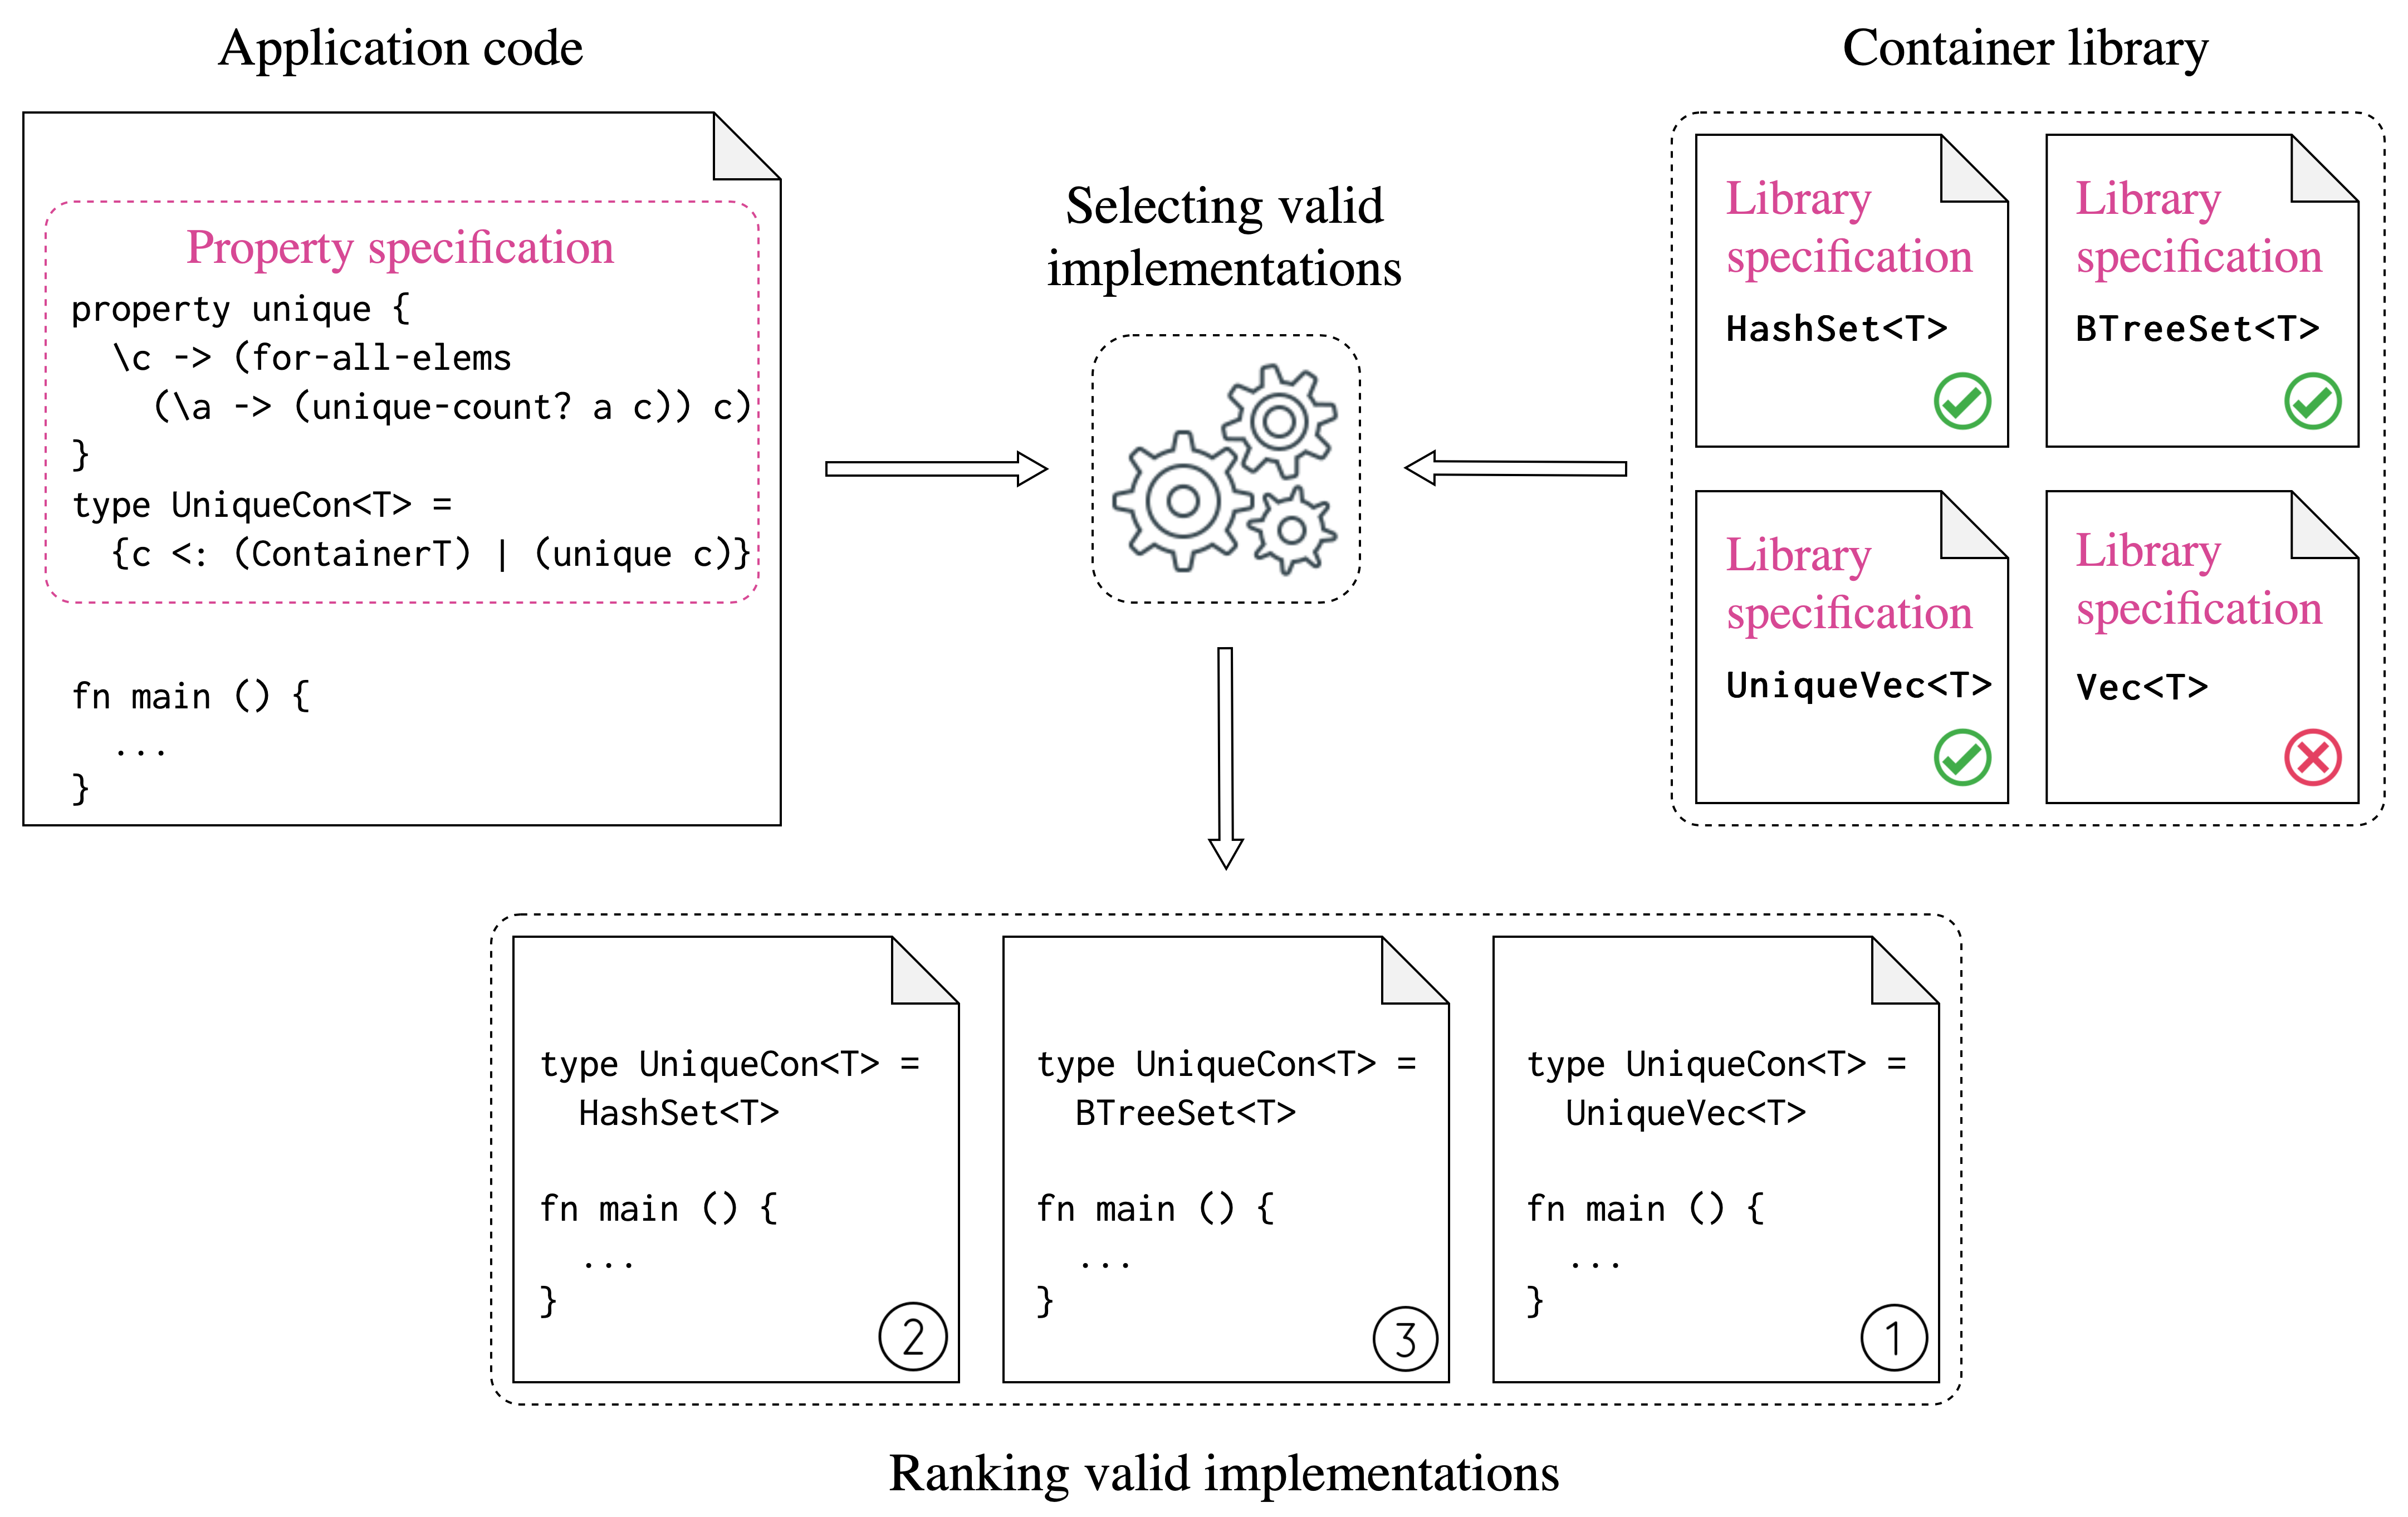
\includegraphics[width=0.95\textwidth]{./overview.png}
    \caption{The workflow of \Primrose{}:
    \emph{Property specifications} (top left), written and used by the application developer, are used to check which \emph{library specifications} (top right), written by library developers, satisfy them.
    Valid implementations (marked with a green check marks), are then ranked by their performance (bottom).
    }
    \label{overview:design}
\end{figure}

Given this code as input, \Primrose{} will, acting as 
a preprocessor, generate copies of the input code where the abstract type is instantiated into a valid concrete implementation that satisfies the expected properties. It determines 
which implementations are valid by consulting \emph{library specifications}, which are provided by library developers. These specifications abstract over concrete container implementations 
and provide a summary of their externally observable semantics. 
For each implementation, the library specification contains the pre- and post-conditions of each operation in terms of an abstract list model. We discuss library specifications in more detail in 
section~\ref{chap2:lib}. 

In our example in 
figure~\ref{overview:design}, the library specification of the \lstinline{Vec<T>} type indicates that it is not a suitable choice for \lstinline{UniqueCon<T>}, as it does not satisfy the required semantic property \lstinline{unique}.
We use a satisfiability modulo theories (SMT) solver for the selection process, which we discuss in section~\ref{chap2:select}.

Figure~\ref{overview:design} shows at the bottom a simplified version of the generated programs. \begin{highlightnew}For each valid concrete implementation, a piece of programs is generated by rewriting a property specification into the container type of a chosen concrete implementation. All generated programs are ranked by \Primrose{} and the application programmer can then pick the best performing one.\end{highlightnew}
Note that in order to make \ref{overview:design} concise, we only show a simplified version of the generated programs with selected implementations that does not reflect how traits constrain available operations for interacting with the container type.
In our implementation, we ensure that only the container operations that the application developer specifies with syntactic properties are accessible in the generated program.
%
% After all valid container implementations are selected, \Primrose{} measures and ranks them according to their performance, and then selects the one providing the best performance for the program.
% We discuss the ranking in \ref{chap2:rank}.
%
Our current prototype of \Primrose{} focuses on ensuring the functional correctness of selecting container implementations based on desired properties.
Nevertheless, we have implemented a simple process that ranks valid implementations by their runtime performance.
Rankings by other non-functional metrics could easily be added to our design.
We provide discussion about code generation and ranking in section~\ref{chap2:rank}.

% Porting to other languages
% We discuss the portability of \Primrose{} in \ref{chap2:evaluation}.
% \paragraph{Using Rosette for Designing Specifications and the Selection Process}
\paragraph*{Using Rosette as the Common Language for Specifications and Selection}
\label{common-language}
The ``solver-aided programming language'' Rosette~\citep{rosette-lang, rosette-paper} is used as the common language in \Primrose{} for the formal parts.
Rosette is chosen for \Primrose{} due to its convenient interface to the Z3 SMT solver and the straightforward translation from \Primrose{} property specifications into Rosette.
Property specifications are used as verification conditions when selecting implementations by checking against library specifications which are directly encoded in Rosette. The selection process is done by interacting with the SMT solver via Rosette.


\paragraph*{Portability of \Primrose{}}
\label{implementation:portability}
Currently, we choose Rust as the target language to implement our idea. Application developers write the property specifications as a part of their Rust programs and \Primrose{} generates Rust code after processing specifications. 
However, \Primrose{} could easily be ported to many other languages, since property specifications, 
library specifications, and the process of selecting implementations are all language-agnostic and not attached to Rust's particular type system or language features.
Adapting property specifications into other languages only requires such languages to have a construct similar to Rust's traits, 
such as traits in Scala and interfaces in Java, allowing us to model syntactic properties. It would be straightforward to add new backends to \Primrose{} to 
generate code in these languages. Our library specifications are, by design, an abstraction over implementation details, describing the intended semantics of container operations without respect to 
their implementation. This means we can trivially adapt these specifications to container libraries from other languages, so long as our specifications remain an abstraction of the 
new implementations.  Thus, we anticipate that \Primrose{} could easily be adapted to produce code in any language with sufficient support for data abstraction, such as Java, Scala, Swift, or \Cpp.

\section{Property Specifications}
\label{chap2:prop}
The application developer specifies the desired behaviours of their required container with a \textit{property specification},
% that consists of \emph{semantic properties}, which refine the container type by a predicate, and \emph{syntactic properties}, which in Rust are traits specifying the operations that must be supported by the container and their types.
%
%The property specification of the type \lstinline{UniqueCon} from the example in \ref{overview:design} is:
for example, for the type \lstinline{UniqueCon} from figure~\ref{overview:design}:
\begin{lstlisting}[language=Rust, style=boxed, escapechar=!]
!\tikz[remember picture, overlay]\node [xshift=12.8cm, yshift=+.075cm, inner sep=0.075cm, rectangle] {\footnotesize\bfseries\texttt{Primrose}};!property unique 
  { \c -> (for-all-elems (\a -> (unique-count? a c)) c) }
type UniqueCon<T> = {c <: (ContainerT) | (unique c)}
\end{lstlisting}

We first define the \emph{semantic property} \lstinline{unique} using a \emph{predicate}.
In our specification language, such predicates have type $\mathit{Con}\langle\tau\rangle \to \mathit{Bool}$, where $\mathit{Con}\langle\tau\rangle$ is a placeholder that is resolved into a concrete container type by 
the selection process. The combinator \lstinline{for-all-elems} is part of a library enabling to write predicates for individual container elements. The predicate \lstinline{unique-count?} holds if and only if the given element occurs exactly once in the container. These combinators and predicates are explained in section~\ref{chap2:prop:semantic}. \begin{highlightnew} One may notice that the predicate \lstinline{unique-count?} relies on equality being able to be done on elements in the container. Currently, a runtime error will be produces if the equality of elements are not defined. We further discuss the potential improvement of such a design in section~\ref{chap2:limitations}.
\end{highlightnew}

With the defined \emph{semantic property} \lstinline{unique}, we can then declare the container type \lstinline{UniqueCon<T>}. 
The first part of the declaration specifies the syntactic property that must be satisfied by the container type, in the form of the trait 
\lstinline{ContainerT}. Specifically, \lstinline{c <: (ContainerT)} says that the type of the container \lstinline{c} must implement the trait \lstinline{ContainerT}, which specifies a set of basic container operations. 
The second part of the declaration \emph{refines} our container type by the predicate \lstinline{unique}, stating that the property must be invariant across all container operations.
Properties may also be composed. For multiple syntactic properties, we specify a list of traits (\lstinline{c <: (T1, T2)}) that the container type implements. For multiple semantic properties, we use conjunction, i.e.\ \lstinline{((p1 c) and (p2 c))}.

\begin{figure}[t]
  \begin{alignat*}{3}
  \mathrm{Literals} \quad 
  &l \ &\metaDef \quad &\mathit{true} \cmid \mathit{false}
  \\[-.25em]
  \mathrm{Terms} \quad
  &t \ &\metaDef \quad &l \cmid x \cmid \lambda x.\ t \cmid t\ t
  \\[-.25em]
  %\mathrm{Predicate} \quad 
  %&p \ &\metaDef \quad &\lambda x.\ t
  %\\[-.25em]
  \mathrm{Refinement} \quad 
  &r \ &\metaDef \quad &t \cmid r \wedge r
  \\[-.25em]
  \mathrm{Container\ Type\ Declarations} \quad 
  &c \ &\metaDef \quad &\{\begin{highlightnew} t \end{highlightnew} \ \metaBound\ B \mid r\}
  \\[-.25em]
  \mathrm{Simple\ Types} \quad 
  &\sigma \ &\metaDef \quad &\mathit{Bool} \cmid T \cmid \mathit{Con}\langle\sigma\rangle 
  \\[-.25em]
  \mathrm{Types} \quad 
  &\tau \ &\metaDef \quad &\sigma \cmid \tau \to \tau \cmid \forall T \metaBound B .\ \tau
  \\[-.25em]
  \mathrm{Bounds} \quad
  &B \ &\metaDef \quad &\mathit{trait\_name} \cmid B \sep B
  %\\[-.25em]
  %\mathrm{Kinds} \quad 
  %&\kappa \ &\metaDef \quad &\mathsf{type} \cmid \kappa_1 \Rightarrow \kappa_2
  \end{alignat*}
  \caption{The syntax of property specifications. $T$ is the type variable, ranging over element types of the target language, which is Rust in this case.}
  \label{prop:syntax}
\end{figure}

Figure~\ref{prop:syntax} shows the syntax of the \Primrose{} property specification language. Formally, the specification language is a variant of the polymorphic $\lambda$-calculus~\citep{DBLP:conf/programm/Reynolds74, DBLP:journals/tcs/Girard86}, with 
restrictions on the use of polymorphism to enable implicit type inference~\citep{hindley1969principal, MILNER1978348}.
This type system guarantees termination, making specifications easier to analyse and straightforward to translate into SMT verification conditions in Rosette.
The translation into Rosette is straightforward, as terms in the \Primrose{} property specification language (literals, variables, lambdas, and function application) are translated into their counterparts in the functional Rosette language.
\begin{lstlisting}[language=Rust, style=boxed, caption={The implementation of a container trait}, label=chap2:prop:syntactic:con-trait, escapechar=!]
!\tikz[remember picture, overlay]\node [xshift=12.95cm, yshift=+.075cm, inner sep=0.075cm, rectangle] {\footnotesize\bfseries\texttt{Rust}};!pub trait ContainerT<T> {
  fn len(&self) -> usize;
  fn contains(&self, x: &T) -> bool;
  fn is_empty(&self) -> bool;
  fn insert(&mut self, elt: T);
  fn clear(&mut self);
  fn remove(&mut self, elt: T) -> Option<T>;}
\end{lstlisting}

\subsection{Syntactic Properties as Traits}
\label{chap2:prop:syntactic}
In our \Primrose{} prototype, we encode syntactic properties as Rust traits, specifying the operations needed by the application developer to interact with a container.
Traits are defined in Rust and lifted into our property specification language. For instance, listing~\ref{chap2:prop:syntactic:con-trait} shows the trait \lstinline|ContainerT| introduced above.

By writing \lstinline{c <: ContainerT}, the application developer indicates that they expect the container type selected by \Primrose{} to include implementations for all operations in the trait \lstinline{ContainerT}. 
Thus, after executing \Primrose{}, \mylstinline{UniqueCon<T>} will be resolved into a concrete container type that implements the trait \lstinline{ContainerT}.

As mentioned, we can also declare a container type that satisfies multiple syntactic properties. For instance, suppose that in addition to \lstinline{ContainerT}, we would like our container to also satisfy the syntactic property \lstinline{IndexableT}:
\begin{lstlisting}[language=Rust, style=boxed, escapechar=!]
!\tikz[remember picture, overlay]\node [xshift=12.95cm, yshift=+.075cm, inner sep=0.075cm, rectangle] {\footnotesize\bfseries\texttt{Rust}};!pub trait IndexableT<T> {
  fn first(&self) -> Option<&T>;
  fn last(&self) -> Option<&T>;
  fn nth(&self, n: usize) -> Option<&T>;
}
\end{lstlisting}

With just \lstinline{ContainerT}, there is no way to observe the \emph{ordering} of elements in the container, but with \lstinline{IndexableT} there is, as we can now select elements based on their position.
By composing our new syntactic property \lstinline{IndexableT} with \lstinline{ContainerT} we can now 
specify a container of unique elements where the order can be observed:
\begin{lstlisting}[language=Rust, style=boxed, escapechar=!]
!\tikz[remember picture, overlay]\node [xshift=12.8cm, yshift=+.075cm, inner sep=0.075cm, rectangle] {\footnotesize\bfseries\texttt{Primrose}};!type UniqueIndexableCon<T> = 
  { c <: (ContainerT, IndexableT) | (unique c) }
\end{lstlisting}

Semantic properties, such as \lstinline{unique}, must be invariant across all operations from all syntactic properties required of the container.
%\todo[author=Michel]{Removed the following snipped, as I think this is redundant}

\subsection{Semantic Properties as Predicates}
\label{chap2:prop:semantic}
As mentioned, semantic properties are predicates that are used to construct refinements for container types; each declared container type in the form $\{v \ \metaBound\ B \mid r\}$ is a \textit{refinement type}, i.e.\ a type circumscribed by a logical predicate~\citep{10.1145/113445.113468}. When the predicates are in SMT-decidable logic, they can be statically checked~\citep{10.1145/1863543.1863560}.
Such techniques are used in programming languages like Liquid Haskell and F*, where they are used to facilitate verification of program correctness. 
For instance, in Liquid Haskell, we may define a refinement type \lstinline{UniqueList} representing a list of unique elements as:
% , caption={Unique List in Liquid Haskell}, captionpos=b, label=prop:lh-uniquelist]
\begin{lstlisting}[language=haskell, style=boxedlst, escapechar=!]
!\tikz[remember picture, overlay]\node [xshift=12.5cm, yshift=+.075cm, inner sep=0.075cm, rectangle] {\footnotesize\bfseries\texttt{Liquid Haskell}};!{-@ measure unique @-}
unique :: (Ord a) => [a] -> Bool
unique [] = True
unique (x:xs) = unique xs && not (S.member x (elts xs))
{-@ type UniqueList a = {v:[a] | unique v} @-}
\end{lstlisting}

\noindent While our syntax for type refinements strongly resembles Liquid Haskell, our refinement types are slightly different, and serve a different purpose.
Firstly, Liquid Haskell's refinements 
are attached to a \emph{concrete type}, in this case a list (written \lstinline{[a]}), whereas our refinements are attached to an abstract container type, which is then resolved by \Primrose{} into a concrete 
implementation. Secondly, Liquid Haskell 
uses type refinements for the purpose of \emph{correctness}: If a list is declared to have type \lstinline{UniqueList}, the Liquid Haskell verifier will check that it satisfies the predicate \lstinline{unique}. 
The \lstinline{notUniqueList} shows that it will report an error at compile time if a given list contains duplicates.
\begin{lstlisting}[language=haskell, style=boxedlst, escapechar=!]
!\tikz[remember picture, overlay]\node [xshift=12.5cm, yshift=+.075cm, inner sep=0.075cm, rectangle] {\footnotesize\bfseries\texttt{Liquid Haskell}};!{-@ notUniqueList :: UniqueList Int @-}
notUniqueList::[Int]
notUniqueList = [3, 1, 2, 3]
\end{lstlisting}
Our work instead uses type refinements to specify the semantic requirements of the application developer to guide selection of valid concrete implementations.
Once all valid implementations have been found, \Primrose{} simply selects the implementation providing the best performance for the application developer.
In short, rather than to aid verification, we use refinement types to help application developers optimise their programs. We give more details on the selection process in section~\ref{chap2:select}.

\paragraph*{Combinators and Predicate Functions} Demonstrated by our examples, \Primrose{} provides a set of combinators and predicate functions to facilitate writing of property specifications. 
These combinators and predicate functions are defined in Rosette and then imported into our property 
specification language.  In the semantic property \lstinline{unique}, the combinator \lstinline{for-all-elems} is used to specify that the predicate \lstinline{unique-count?} must hold for all elements inside the container. 
The type of the combinator \lstinline{for-all-elems} is $\mathit{Con}\langle\tau\rangle \to (\tau \to \mathit{Bool}) \to \mathit{Bool}$, meaning this combinator takes in two arguments, the first of which is a container and the second of which is a predicate on the elements of that container, and eventually returns a boolean value.

For the purposes of checking, we represent containers $\mathit{Con}\langle\tau\rangle$ abstractly in Rosette as lists. We discuss this list abstraction and justify it in section~\ref{chap2:lib}.
With such a list abstraction, we are able to straightforwardly implement our \lstinline{for-all-elems} combinator with a list fold operation:
\begin{lstlisting}[language=racket, style=boxed, label=prop:combinator-unary, escapechar=!] 
!\tikz[remember picture, overlay]\node [xshift=12.8cm, yshift=+.075cm, inner sep=0.075cm, rectangle] {\footnotesize\bfseries\texttt{Rosette}};!(define (for-all-elems c fn)
    (foldl elem-and #t (map (lambda (a) (fn a)) c)))
\end{lstlisting}

We also provide some combinators for applying \emph{relations} between elements in a container. For instance, the combinator \mylstinline{for-all-consecutive-pairs}:
\begin{align}
    \label{prop:combinator-pair}
    \texttt{for-all-consecutive-pairs}\; :\; \mathit{Con}\langle\tau\rangle \to (\tau \to \tau \to \mathit{Bool}) \to \mathit{Bool}
\end{align}
Unlike \lstinline{for-all-elems}, this combinator gives a binary relation between elements, and checks that this relation holds between any two consecutive elements in a container.

With the combinator \lstinline{for-all-consecutive-pairs} and the predicates \lstinline{geq?} and \lstinline{leq?}, we can define properties like \lstinline{ascending} and \lstinline{descending}, which specify particular orderings of elements in a container:
\begin{lstlisting}[language=Rust, style=boxed, escapechar=!]
!\tikz[remember picture, overlay]\node [xshift=12.8cm, yshift=+.075cm, inner sep=0.075cm, rectangle] {\footnotesize\bfseries\texttt{Primrose}};!property ascending { \c -> (for-all-consecutive-pairs c leq?) }
property descending { \c -> (for-all-consecutive-pairs c geq?) }
\end{lstlisting}

Besides the set of combinators and predicate functions predefined in \Primrose{}, application developers may also provide customised functions by providing Rosette definitions and importing them into our property specification language. 

\paragraph*{Composition of semantic properties} As shown in figure~\ref{prop:syntax}, we can compose semantic properties in a container type declaration with conjunction.
For instance, to declare a container type with elements arranged in \emph{strictly} ascending order, i.e., both \lstinline{unique} and \lstinline{ascending} properties must hold, we can write the following:
\begin{lstlisting}[language=Rust, style=boxed]
!\tikz[remember picture, overlay]\node [xshift=12.8cm, yshift=+.075cm, inner sep=0.075cm, rectangle] {\footnotesize\bfseries\texttt{Primrose}};!type StrictlyAscendingCon<T> = 
  { c <: (ContainerT) | ((unique c) and (ascending c)) }
\end{lstlisting}
The conjunction \lstinline|and| is directly translated into a conjunction operation in Rosette.

\subsection{The \begin{highlightnew}Dependencies\end{highlightnew} between Semantic Properties and Syntactic Properties}
\label{chap2:prop:semantic-syntactic}
All semantic properties we have seen so far have been invariants across all operations, but 
some semantic properties relate to specific operations given by syntactic properties. 
For instance, when specifying a stack container type providing operations \lstinline{push} and \lstinline{pop} with the expected last-in-first-out (LIFO) property.
% on top of the trait \lstinline{ContainerT} specifying basic container operations, 
Firstly, we define a trait specifying operations \lstinline{push} and \lstinline{pop}, namely \lstinline{StackT}:
\begin{lstlisting}[language=Rust, style=boxed, caption=The trait \mylstinline{StackT} specifying operations \mylstinline{push} and \mylstinline{pop}, captionpos=t, label=prop:spec-stackt, escapechar=!]
!\tikz[remember picture, overlay]\node [xshift=12.95cm, yshift=+.075cm, inner sep=0.075cm, rectangle] {\footnotesize\bfseries\texttt{Rust}};!pub trait StackT<T> {
  fn push(&mut self, elt: T);
  fn pop(&mut self) -> Option<T>;
}
\end{lstlisting}
Secondly, we define the semantic property \lstinline{lifo} for containers that implement \lstinline{StackT}:
\begin{lstlisting}[language=Rust, style=boxed, caption=The semantic property LIFO, captionpos=t, label=prop:spec-lifo, escapechar=!]
!\tikz[remember picture, overlay]\node [xshift=12.8cm, yshift=+.075cm, inner sep=0.075cm, rectangle] {\footnotesize\bfseries\texttt{Primrose}};!property lifo { \c <: StackT -> (forall \x. pop (push c x) == x) }
\end{lstlisting}
\noindent
Unlike previously, this semantic property includes a requirement that the given container implements the trait \lstinline{StackT}, enabling us to refer to the operations \lstinline{pop} and \lstinline{push} inside the semantic property. In this definition, \lstinline{forall} is a combinator with type:
\begin{align}
    \label{prop:combinator-forall}
    \texttt{forall}\; :\; \forall x. \,(x \to \mathit{Bool}) \to \mathit{Bool}
\end{align}
This combinator is implemented with the \lstinline{forall} procedure defined in Rosette's library, which serves as a construct for creating universally quantified formulae.

Armed with the trait \lstinline{StackT} and the semantic property \lstinline|lifo|, we can combine all these elements and declare our stack type as follows:
%  caption=The container type with stack operations satisfying the semantic property LIFO, captionpos=b,
\begin{lstlisting}[language=Rust, style=boxed, escapechar=!]
!\tikz[remember picture, overlay]\node [xshift=12.8cm, yshift=+.075cm, inner sep=0.075cm, rectangle] {\footnotesize\bfseries\texttt{Primrose}};!type StackCon<T> = {c <: (ContainerT, StackT) | (lifo c)}
\end{lstlisting}

In the next section, we will discuss how library developers write specifications for their container implementations.

%\Primrose{} selects among these library specifications the ones that satisfy the properties required by application developers.

\section{Library Specifications}
\label{chap2:lib}
% show full spec
% unique + lifo
% verification
% no good rust semantic framework for verification yet; rust belt in dev.
%
% TODO: Should we remove this to streamline the presentation (this feels a bit like a re-motivation of the points we made already in the introduction)
% It is not feasible to select container implementations directly by analysing their Rust source code and checking if they satisfy the properties specified by the application developer.
% Rust is a Turing-complete, general purpose programming language with a complex semantics, and its container libraries 
% are typically highly optimised, making extensive use of unsafe code. Doing such a broad analysis precisely and automatically is very hard even for the most advanced of static analyses.
% Instead, we write 
\emph{Library specifications} abstract over Rust container implementations, providing a clear definition of intended semantics of each operation, without respect to performance or implementation details. 
This approach allows us to select container implementations by simply checking their library specifications, rather than their full implementations, against the properties specified by the application developer.
Moreover, using specifications which are abstracted from implementations makes \Primrose{} easy to repurpose for programming languages other than Rust, as the same specifications would apply, with minimal or no modification, to container libraries written in any other language. 

By encoding these specifications into \emph{property based tests}, which validate container implementations against their library specifications (section~\ref{chap2:evaluation:testing}), we ensure the selected implementations indeed satisfy a required property specification. Since these library specifications form a \emph{functional correctness} specification for each operation, they could also be used in future as the basis of full functional correctness verification with a verification framework for Rust~\citep{rustbelt-paper}, but this is out of scope for \Primrose{}.

\subsection{The Basic Design of Library Specifications}
\label{chap2:lib:design}
Library specifications of concrete container implementations are developed based on Hoare logic~\citep{10.1145/363235.363259}.
For each concrete container implementation, we provide a set of \emph{Hoare triples}, one for each operation. A Hoare triple of the form
$\{\phi\}\; \mathsf{op} \;\{\psi\}$ states that if the \textit{precondition} $\phi$ holds and the operation $\mathsf{op}$ is executed, then the \textit{postcondition} $\psi$ will hold.
These conditions are predicates on the state of the program. In our case, the state contains the container, plus any other inputs and outputs of the operation $\mathsf{op}$.

As mentioned in section~\ref{chap2:overview}, we model the container as a list in Rosette for \Primrose{}'s library specifications. The list is a model to convey the intended semantics, and does not proscribe anything about the implementation --- the implementation is free to represent 
data in any chosen structure. For example, a set data type may be implemented with a binary search tree, but will still be specified with a list. 
These model lists are a simple abstraction, easy to analyse, with which all container operations can be specified.

\paragraph*{Library Specifications Convey the Intended Semantics for Implementations} It is important that all possible executions of a concrete implementation should be captured by its library specification. Otherwise in the process of selecting implementations by checking if their library specifications match the required semantic property, \Primrose{} could select an unsatisfying implementation. More formally, a proof of functional correctness of an implementation w.r.t. its specification would take the form of a data refinement~\citep{de_roever_engelhardt_1998},
where each value of the concrete container type is related to our list model by an \emph{abstraction function} $\alpha$, and our specification on lists is shown to contain all possible behaviours 
of the concrete implementation using a \emph{forward simulation}:
% \begin{figure}[!ht]
\vspace{-.5em}
\begin{center}
  $\begin{array}{c}\alpha^{-1};\mathsf{op(\textit{C})}  \subseteq
  \mathsf{op(\textit{A})}; \alpha^{-1}\quad\\\text{\footnotesize (where ; is forward composition of relations} \\\text{\footnotesize and $\alpha^{-1}$ is the inverse relation of $\alpha$)}\end{array}$
\begin{tikzcd}[row sep=1.2cm,column sep=1.2cm,inner sep=0.7ex, cramped]
\circ
\arrow[Mapsto]{r}[name=U]{\textsf{op(\textit{A})}}
\arrow[dr, rounded corners,
       to path={ ([xshift=1.3ex,yshift=-0.5ex]\tikztostart.south) |- ([yshift=1.3ex,xshift=-0.5ex]\tikztotarget.west)}]
\arrow[dr, rounded corners,
       to path={ ([yshift=-1.3ex,xshift=0.5ex]\tikztostart.east) -| ([xshift=-1.3ex, yshift=0.5ex]\tikztotarget.north)}]
&
\circ
\\
\bullet
\arrow[dashed]{u}{\alpha}
\arrow[swap, Mapsto]{r}[name=D]{\textsf{op(\textit{C})}}
&
\bullet
\arrow[swap,dashed]{u}{\alpha}
\arrow[to path={(U) node[midway,scale=1.5] {\rotatebox[origin=c]{90}{$\subseteq$}}  (D)}]{}
\end{tikzcd}
\end{center}
% \caption{Forward simulation} \label{lib:forward-simulation}
% \end{figure}

\noindent Here, $\mathsf{op(\textit{C})}$ denotes the concrete implementation of our operation $\mathsf{op}$, represented as a relation from inputs to outputs.
The abstract operation $\mathsf{op(\textit{A})}$ is the maximal relation satisfying the Hoare triple given in our library specification, and $\alpha$ is a suitable abstraction function that 
flattens a concrete container into a list. 

If a forward simulation is shown for all operations, we can then conclude that each possible execution with the concrete container implementation has a corresponding execution with an abstract list, thus the specification accurately captures the implementation's semantics.

For instance, a binary search tree $T$ can be abstracted to a sorted list $L$ by an abstraction function $\mathit{inorder}$ that does an in-order traversal. For each operation interacting with $T$, there exists a corresponding operation at the abstract level defined using $L$. 
Take the operation $\mathsf{insert(\textit{T},x)}$, which inserts an element $x$ into a binary search tree $T$. We can abstract such an operation to $\mathsf{insert(\textit{L},x)}$ which inserts $x$ at the right location in a sorted list. The relation between these two operations is shown by this diagram:
\vspace{-.4em}
\begin{center}
 % $\begin{array}{c}\mathit{inorder}(\mathsf{insert}(\textit{T},x)) \mathit{inorder}^{-1};\mathsf{len(\textit{T})}  \subseteq
 % \mathsf{len(\textit{L})}; inorder^{-1}\quad\end{array}$
\begin{tikzcd}[row sep=1.2cm,column sep=1.2cm,inner sep=0.7ex, cramped]
\circ
\arrow[Mapsto]{r}[name=U]{\textsf{insert(\textit{L},x)}}
\arrow[dr, rounded corners,
       to path={ ([xshift=1.3ex,yshift=-0.5ex]\tikztostart.south) |- ([yshift=1.3ex,xshift=-0.5ex]\tikztotarget.west)}]
\arrow[dr, rounded corners,
       to path={ ([yshift=-1.3ex,xshift=0.5ex]\tikztostart.east) -| ([xshift=-1.3ex, yshift=0.5ex]\tikztotarget.north)}]
&
\circ
\\
\bullet
\arrow[dashed]{u}{\mathit{inorder}}
\arrow[swap, Mapsto]{r}[name=D]{\textsf{insert(\textit{T},x)}}
&
\bullet
\arrow[swap,dashed]{u}{\mathit{inorder}}
\arrow[to path={(U) node[midway,scale=1.5] {\rotatebox[origin=c]{90}{$\subseteq$}}  (D)}]{}
\end{tikzcd}
\end{center}
\vspace{-.4em}
\noindent In this work, we specified four container implementations from Rust's standard library (\lstinline!Vec!,\,\lstinline!LinkedList!,\,\lstinline!HashSet!,\,\lstinline!BTreeSet!) and four custom container implementations (\lstinline!SortedVec!,\,\lstinline!LazySortedVec!,\,\lstinline!UniqueVec!,\,\lstinline!LazyUniqueVec!) by abstracting them into a list model.
As we discuss in section~\ref{chap2:lib:abstracting}, library specifications abstract over some implementation details, and, thus, \lstinline!Vec! and \lstinline!LinkedList! share the same specifications, as do the eager and lazy \lstinline!SortedVec! and \lstinline!UniqueVec! implementations.
For each specification, we define a suitable abstraction function for forward simulation which, while not needed for selection, is used for property-based testing to justify that a concrete implementation satisfies the intended semantics described by its library specification.

\paragraph*{Completeness of Library Specifications} 
While it is important to ensure that library specifications indeed convey the intended semantics of the implementation, \emph{completeness} of library specifications is also important. Without completeness, \Primrose{} could possibly rule out perfectly valid implementations because it cannot prove that the required semantic properties are preserved for an operation of which the specification is incomplete. \begin{highlightnew}For instance, specifying a \verb|BTreeSet| which is a concrete container implementation that contains unique elements sorted in ascending order with a model that is a sorted but not unique list would be incomplete. With such an incomplete specification, although a \verb|BTreeSet| is a valid strictly ascending container, it will be ruled out by \Primrose{} since its library specification does not satisfy the property \verb|StrictlyAscendingCon|. \end{highlightnew}

Our approach easily ensures completeness when each operation is specified by a \emph{deterministic} model operation. Forward simulation states that every execution of the concrete implementation has a corresponding execution in the abstract operation, while determinism states that such correspondence is one-to-one, i.e., each abstract execution also has a corresponding concrete one.
Thus, just as forward simulation states that each property established for an abstract operation applies also (via the inverse of the abstraction function $\alpha^{-1}$) to a concrete implementation, completeness states that each property established for a concrete implementation applies (via the abstraction function $\alpha$) to the abstract operation. With both completeness and forward simulation, we ensure that \emph{all} valid implementations and \emph{only} the valid implementations are selected by \Primrose{}.

There are many other available approaches for modelling library specifications, for instance, the axiomatic approach used in algebraic specifications for abstract data types \cite{WIRSING1990675}, specifying the behaviour of operations as a set of equational axioms that relate various operations.
However, it is hard to ensure the completeness of algebraic specifications, as it is hard capture all behaviours of all operations by a set of equations.  

\subsection{The Library Specification of A \texttt{LinkedList}}
\label{chap2:lib:list}
Rust's \lstinline{LinkedList} is a doubly-linked list. The abstraction function to convert it into a logic list is straightforward: Collect all nodes' values with previous and next pointers.

Firstly, we specify the insertion operation, \lstinline|LinkedList::insert|, of which the type signature is:
% caption=The signature of \mylstinline{LinkedList::insert}, captionpos=b, label=lib:sig-list-insert
\begin{lstlisting}[language=Rust, style=boxed, escapechar=!]
!\tikz[remember picture, overlay]\node [xshift=12.95cm, yshift=+.075cm, inner sep=0.075cm, rectangle] {\footnotesize\bfseries\texttt{Rust}};!fn insert(&mut self, elt: T) {...}
\end{lstlisting}
\noindent
Since variables in Rosette are immutable, in the corresponding abstract insertion operation, we alter the type to return a new list instead of altering the list in-place\footnote{Rosette is untyped, but this is morally the type signature.}:
%, caption=The signature of the abstract operation corresponding to \mylstinline{LinkedList::insert}, captionpos=b, label=lib:sig-abs-insert
\begin{lstlisting}[language=racket, style=boxed]
!\tikz[remember picture, overlay]\node [xshift=12.8cm, yshift=+.075cm, inner sep=0.075cm, rectangle] {\footnotesize\bfseries\texttt{Rosette}};!abs-insert: List<T> -> T -> List<T>
\end{lstlisting}
We can then provide the specification of \lstinline|LinkedList::insert| with respect to its corresponding abstract operation, the maximal relation satisfying the Hoare triple:
\begin{align}
\label{lib:spec-list-insert}
\{xs_0.\ \texttt{\small true}\}~\texttt{abs-insert}~\{xs_0\ x\ xs.\ xs = \texttt{\small model-insert}\ xs_0\ x\}
\end{align}
Here, $xs_0$ refers to the initial value of the container, $xs$ refers to the resultant container, and $x$ is the element we insert. The function \lstinline|model-insert| is defined in Rosette on lists:
%, caption=The model insertion operation, captionpos=b, label=lib:logic-list-insert
\begin{lstlisting}[language=racket, style=boxed]
!\tikz[remember picture, overlay]\node [xshift=12.8cm, yshift=+.075cm, inner sep=0.075cm, rectangle] {\footnotesize\bfseries\texttt{Rosette}};!(define (model-insert xs x) (append xs (list x)))
\end{lstlisting}
The postcondition states that we expect applying the insertion operation to a container to produce the same result as the result produced by \lstinline|model-insert| function. In library specifications, defining such \emph{model operations} is a common technique to simplify writing postconditions. 

Similarly, we also provide the specification for the operation \lstinline{LinkedList::contains}:
%, caption=The signature of \mylstinline{LinkedList::contains}, captionpos=b, label=lib:sig-list-contains
\begin{lstlisting}[language=Rust, style=boxed, escapechar=!]
!\tikz[remember picture, overlay]\node [xshift=12.95cm, yshift=+.075cm, inner sep=0.075cm, rectangle] {\footnotesize\bfseries\texttt{Rust}};!fn contains(&self, x: &T) -> bool {...}
\end{lstlisting}
\noindent
In our corresponding abstract operation, in addition to the boolean value indicating whether the given element \lstinline|x| is present or not, the input container is also returned, as we would like to express the input container is not mutable, its value remains unchanged after this operation. Also, since the underlying value with type \lstinline|T| is given by an immutable reference \lstinline|&T|, in the abstract operation we treat the immutable reference \lstinline|&T| as simply \lstinline|T|. The signature of the abstract operation is shown below:
\begin{lstlisting}[language=racket, style=boxed, caption=The signature of the abstract operation corresponding to \mylstinline{LinkedList::contains}, captionpos=t, label=lib:sig-abs-contains]
!\tikz[remember picture, overlay]\node [xshift=12.8cm, yshift=+.075cm, inner sep=0.075cm, rectangle] {\footnotesize\bfseries\texttt{Rosette}};!abs-contains: List<T> -> T -> (List<T>, bool)
\end{lstlisting}
The Hoare triple that serves as the specification of \lstinline|LinkedList::contains| is:
\begin{align}
\label{lib:spec-list-contains}
\{xs_0.\ \texttt{\small true}\}\ \texttt{abs-contains}\ \{xs_0\ x\ xs\ r.\ (xs, r) = \texttt{\small model-contains}\ xs_0\ x\}
\end{align}
Note that in this specification, the model operation \lstinline|model-contains| defined in listing~\ref{lib:logic-list-contains} has the same type signature as the abstract operation shown in listing~\ref{lib:sig-abs-contains}. It also returns a pair of values: the output list, which is always equal to the input list, and a boolean value indicating if the element is present in the list.
\begin{lstlisting}[language=racket, style=boxed, caption=The model operation for checking an element's containment, captionpos=t, label=lib:logic-list-contains]
!\tikz[remember picture, overlay]\node [xshift=12.8cm, yshift=+.075cm, inner sep=0.075cm, rectangle] {\footnotesize\bfseries\texttt{Rosette}};!(define (model-contains xs x)
  (cond [(list? (member x xs)) (cons xs #t)]
        [else (cons xs #f)]))
\end{lstlisting}
Because \lstinline|model-contains| returns the unchanged list, it specifies that the operation \lstinline|LinkedList::contains| should not change the list. 

The library specification of the list removal operation is slightly more complicated, we use \lstinline|T?| to denote that a type may be \lstinline|null| to express Rust's \lstinline{Option<T>} type, which is the return type of \lstinline|LinkedList::remove|. 
The type signature of \lstinline|LinkedList::remove| is shown below:
%, caption=The type signature of \mylstinline{LinkedList::remove}, captionpos=b, label=lib:sig-list-remove
\begin{lstlisting}[language=Rust, style=boxed, escapechar=!]
!\tikz[remember picture, overlay]\node [xshift=12.95cm, yshift=+.075cm, inner sep=0.075cm, rectangle] {\footnotesize\bfseries\texttt{Rust}};!fn remove(&mut self, x: T) -> Option<T> {...}
\end{lstlisting}
\noindent
This operation removes the first occurrence of an element from the given linked list and returns it. If the linked list does not contain the element, \lstinline|None| is returned and the list remains unchanged.
The signature of the corresponding abstract operation is:
%, caption=The signature of the abstract operation corresponding to \mylstinline{LinkedList::remove}, captionpos=b, label=lib:sig-abs-remove
\begin{lstlisting}[language=racket, style=boxed]
!\tikz[remember picture, overlay]\node [xshift=12.8cm, yshift=+.075cm, inner sep=0.075cm, rectangle] {\footnotesize\bfseries\texttt{Rosette}};!abs-remove: List<T> -> T -> (List<T>, T?)
\end{lstlisting}
The model removal operation has the same signature as the abstract operation. We return \lstinline|null| in Rosette for the \lstinline|None| case:
%, caption=The model removal operation, captionpos=b, label=lib:logic-list-remove
\begin{lstlisting}[language=racket, style=boxed]
!\tikz[remember picture, overlay]\node [xshift=12.8cm, yshift=+.075cm, inner sep=0.075cm, rectangle] {\footnotesize\bfseries\texttt{Rosette}};!(define (model-remove xs x) 
  (cond [(list? (member x xs)) (cons (remove x xs) x)]
        [else (cons xs null)]))
\end{lstlisting}
Again, we return a pair of the resulting list and the element being removed. Then we provide the library specification of \lstinline|LinkedList::remove|:
\begin{align}
\label{lib:spec-list-remove}
\{xs_0.\ \texttt{\small true}\}\ \texttt{abs-remove}\ \{xs_0\ x\ xs\ r.\ (xs, r) = \texttt{\small model-remove}\ xs_0\ x\}
\end{align}
To provide a complete specification of \lstinline|LinkedList|, the library developer must ensure that each operation of the \lstinline|LinkedList| is specified by a trait, and for each operation in each trait the \lstinline|LinkedList| implements, specifications similar to the above are provided.

\subsection{The Library Specification of A \texttt{BTreeSet}}
\label{chap2:lib:btree}
For the \lstinline|LinkedList| it is intuitive to use a logic list as a model, as they are both lists. However, even for non-linear structures such as trees, we can still use logic lists as a model. 
Rust's \lstinline|BTreeSet| is a set implemented using a b-tree.
All elements are unique and arranged in ascending order. Thus, our list model of the b-tree is simply a sorted list in ascending order, where uniqueness of elements is preserved.
The abstraction function $\alpha$ that converts the \lstinline|BTreeSet| to our list model is simply an in-order traversal.

The first example to be illustrated is again the specification of the insertion operation with signature:
%, caption=The signature of \mylstinline{BTreeSet::insert}, captionpos=b, label=lib:sig-tree-insert
\begin{lstlisting}[language=Rust, style=boxed, escapechar=!]
!\tikz[remember picture, overlay]\node [xshift=12.95cm, yshift=+.075cm, inner sep=0.075cm, rectangle] {\footnotesize\bfseries\texttt{Rust}};!pub fn insert(&mut self, value: T) {...}
\end{lstlisting}
\noindent
The signature of the abstract insert operation on our model lists is the same as for \lstinline{LinkedList::insert}.
% resembles the abstraction of \lstinline{LinkedList::insert}:
%, caption=The signature of the abstract operation corresponding to \mylstinline{BTreeSet::insert}, captionpos=b, label=lib:sig-abs-insert-tree
% \begin{lstlisting}[language=racket, style=boxed]
% abs-insert: List<T> -> T -> List<T>
% \end{lstlisting}
The specification of \lstinline{abs-insert} for \lstinline|BTreeSet|, however, differs from that of \lstinline|LinkedList|, as we must maintain ordering and uniqueness of elements:
\begin{align}
\label{lib:spec-tree-insert}
\{xs_0.\ xs_0 = \texttt{\small dedup}\ (\texttt{\small sort}\ xs_0\ \texttt{\small<})\}~\texttt{abs-insert}~\{xs_0\ x\ xs.\ xs = \texttt{\small model-insert}\ xs_0\ x\}
\end{align}
Again, $x$ is the element to be inserted, and $xs_0$ and $xs$ are lists modelling the container (via the in-order traversal function $\alpha$) before and after the \lstinline|abs-insert| operation respectively. 
We place an assertion $xs_0 = \texttt{\small dedup}\ (\texttt{\small sort}\ xs_0\ \texttt{\small<})$ in the precondition requiring that the model $xs_0$ to be a sorted list of unique elements. 
While this precondition should always be satisfied by an in-order traversal of a valid b-tree, we do not want our abstraction to constrain the implementation's behaviour if the data invariants of the b-tree are violated --- given a malformed b-tree, the 
implementation should be free to return any result. Because the semantics of \lstinline{abs-insert} are the maximal relation satisfying this specification, this abstract operation contains all possible behaviours of the concrete implementation if this precondition is violated. The \lstinline|model-insert| here is simply an insertion operation defined on a sorted list of unique elements:
%, caption=The unique and sorted list's model insertion operation, captionpos=b, label=lib:unique-sorted-list-insert
\begin{lstlisting}[language=racket, style=boxed]
!\tikz[remember picture, overlay]\node [xshift=13.0cm, yshift=+.075cm, inner sep=0.075cm, rectangle] {\footnotesize\bfseries\texttt{Rosette}};!(define (model-insert xs x) (dedup (sort (append xs (list x)) <)))
\end{lstlisting}
% \todo[author=XY]{I guess we don't need to talk about the efficiency here?} (Michel: Agree)
% Note that because our specifications do not need to be efficient, we can na\"ively implement this function simply by appending the new element to the list, then sorting and removing duplicates from it.

We can also provide specifications for abstract operations that observe the ordering of elements in a \lstinline|BTreeSet|, such as those operations from the \lstinline|IndexableT| trait, since there is a one-to-one correspondence between each element's position in a \lstinline|BTreeSet| and its position in the model list abstracted from the \lstinline|BTreeSet|.
For instance, we provide the specification of the operation \lstinline|BTreeSet::first|, which is the operation obtaining the first (and also the minimal) element of a \lstinline|BTreeSet| with signature:
%, caption=The signature of \mylstinline{BTreeSet::first}, captionpos=b, label=lib:sig-tree-first
\begin{lstlisting}[language=Rust, style=boxed, escapechar=!]
!\tikz[remember picture, overlay]\node [xshift=12.95cm, yshift=+.075cm, inner sep=0.075cm, rectangle] {\footnotesize\bfseries\texttt{Rust}};!fn first(&self) -> Option<&T> {...}
\end{lstlisting}
\noindent
We again provide the signature of its corresponding abstract operation:
%, caption=The signature of the abstract operation corresponding to \mylstinline{BTreeSet::first}, captionpos=b, label=lib:sig-abs-first-tree
\begin{lstlisting}[language=racket, style=boxed]
abs-first: List<T> -> (List<T>, T?)
\end{lstlisting}
Like \lstinline|LinkedList::contains| in listing~\ref{lib:sig-abs-contains}, this type includes a returned list, as \Primrose{} does not consider the immutability of \lstinline|&self| in the Rust type signature above. 
We again include the requirement that the container is unchanged in the specification:
\begin{align}
\label{lib:spec-tree-first}
\{xs_0.\ xs_0 = \texttt{\small dedup}\ (\texttt{\small sort}\ xs_0\ \texttt{\small<})\}~\texttt{abs-first}~\{xs_0\ xs\ x.\ (xs, x) = \texttt{\small model-first}\ xs_0\}
\end{align}
Here, \lstinline|model-first| is defined as a function that returns the first element of the list, is present, along with the list itself:
%, caption=The model operation obtaining the first element of a list, captionpos=b, label=lib:unique-sorted-list-first
\begin{lstlisting}[language=racket, style=boxed]
!\tikz[remember picture, overlay]\node [xshift=12.8cm, yshift=+.075cm, inner sep=0.075cm, rectangle] {\footnotesize\bfseries\texttt{Rosette}};!(define (model-first xs) 
  (cond 
    [(null? xs) (cons xs null)] 
    [else (cons xs (first xs))]))
\end{lstlisting}
% (define (model-first xs)
%   (cond
%     [(null? xs) (cons xs null)]
%     [else (cons xs (first xs))]))
As before, our precondition includes the assumption that the model $xs_0$ abstracted from the \lstinline{BTreeSet} contains unique elements that are sorted in ascending order. 

\subsection{The Library Specification of A \texttt{HashSet}}
\label{lib:hashset}
A tree implementation of a set maintains its elements in a fixed ascending order, and the ordering of our abstract list model simply reflects the ordering of the elements in the tree. However, some container implementations
do not have a fixed ordering of elements. For instance, the \lstinline|HashSet| in Rust is a set implementation 
using a hash algorithm which is randomly seeded. Despite the implementation storing elements in an unspecified order, we may still safely 
use a sorted, ascending list of unique elements as our abstract model of a \lstinline|HashSet|: Our abstraction function $\alpha$ merely collects all elements from the \lstinline|HashSet| into a list and then sorts them into ascending order.

Since the ordering of elements in our list is now different from the ordering of elements in the \lstinline|HashSet|, the developer may specify 
properties relating to the ordering of elements, such as \lstinline|ascending|, that are not satisfied by the implementation, but are trivially satisfied by the 
abstraction function. This would lead to \lstinline|HashSet| being considered a valid choice for an \lstinline|ascending| container.
However, \Primrose{} prevents this by the checking of syntactic properties. The \lstinline|HashSet| type does not implement any trait with operations that allow the ordering of its elements to be observed. 

Therefore, in applications for which the ordering of elements is important, \lstinline|HashSet| is never a valid choice. The selection process of valid implementations according to traits is discussed in section~\ref{chap2:select:syntactic}. 

If a library developer decides to write a \lstinline|HashSet| with operations that leak ordering, they can provide a nondeterministic library specification for such a HashSet that can still be used by Primrose in the selection process.

For the operations defined on \lstinline|HashSet| and \lstinline|BTreeSet|, such as \lstinline|insert|, \lstinline|remove| and \lstinline|contains|,
 the specifications of both implementations are identical---after all, the only observable difference between the implementations is performance---but 
 the specification for \lstinline|HashSet| lacks operations that observe the ordering of its elements, such as \lstinline|first| or \lstinline|last|.

\subsection{Abstracting Over Implementation Details with Library\\Specifications}
\label{chap2:lib:abstracting}
Since the basic container operations of both \lstinline|HashSet| and \lstinline|BTreeSet| have the same externally observable behaviour, we can use the same specifications for both implementations.
There are many such cases where specifications can be re-used: For instance, we provide two implementations of an ascending vector: \lstinline{SortedVec} and \lstinline{LazySortedVec}. \lstinline{SortedVec} maintains the ascending order of elements inside the vector on insertion (\emph{eager}) and \lstinline{LazySortedVec} instead sorts elements whenever the vector is accessed (\emph{lazy}). 
Since both implementations share the same externally observable behaviour, we use the same model for both implementations: A list with elements sorted in ascending order.
Also, their operations are specified with the same set of model operations.
For the eager implementation, the abstraction function $\alpha$ simply collects all its elements into a list. For the lazy implementation, in addition to collecting all elements into a list, the abstraction function $\alpha$ also sorts elements into ascending order.

%These examples demonstrate that our library specifications form a concise model that abstracts over any implementation details that would complicate the process of selecting valid implementations. 
%We further conjecture that these specifications and abstraction functions would have a valid forward simulation to any correct implementation, but due to lack of verification framework in Rust, 
%this conjecture cannot yet be confirmed. Thus, it remains the responsibility of the library developer to provide valid library specifications that accurately describe the behaviour of their implementation.

% \subsection{Completeness of Library Specifications}
% \label{lib:complete}
 
% Soundness of these specifications, which we have ensured via property-based testing, is crucial to guarantee that \Primrose{} does not select implementations which do not satisfy the required semantic properties. 
% However, \emph{completeness} of these specifications is also important. Without completeness, it would be possible that \Primrose{} could rule out perfectly valid implementations because 
% it cannot prove that the required semantic properties are preserved for an incompletely-specified operation. 

% Our approach easily ensures completeness when each operation is specified by a \emph{deterministic} model operation. Soundness tells us that every execution of the concrete implementation has a corresponding execution in the abstract operation, while determinism tells us that this correspondence is one-to-one, meaning that 
% each abstract execution also has a corresponding concrete one.
% Thus, just as soundness states that each property established for an abstract operation applies also (via the inverse of the abstraction function $\alpha^{-1}$) to a concrete implementation, we have \emph{completeness}, stating that each property established for a concrete implementation applies (via the abstraction function $\alpha$) 
% to the abstract operation. With both completeness and soundness, we ensure that \emph{all} valid implementations and \emph{only} the valid implementations are selected by \Primrose{}.

% There are many other approaches we could have taken for modelling library specifications.
% For instance, the axiomatic approach used in algebraic specifications for abstract data types \cite{WIRSING1990675}, which specifies the behaviour of operations by using a set of equational axioms that relate various operations.
% However, it is difficult to ensure the completeness of algebraic specifications, as it is difficult to ensure all behaviours of all operations are captured by a set of equations.  

%We have seen how properties are specified by application developers as traits and type refinements, and how container implementations are specified by library developers as Hoare triples.
%Next, we will discuss how \Primrose{} selects among all library specifications the valid implementations that satisfy the desired properties.

\section{Selecting and Ranking Implementations}
\label{chap2:select}
Before ranking container implementations by performance or other non-functional metrics, \Primrose{} must first identify all implementations that comply
with the property specifications provided by the application developer.
% This selection process comprises two steps: Firstly, \Primrose{} selects all container implementations that satisfy the required \emph{syntactic} properties. Secondly, from the implementations selected in the first step, it selects the ones whose library specifications match the required \emph{semantic} properties.
% The first step is accomplished by simply gathering all types that implement the required Rust traits. For the second step, we check semantic properties against library specifications using the SMT solver in the backend of Rosette.

\subsection{Selecting Container Implementations Satisfying Syntactic Properties}
\label{chap2:select:syntactic}
The first step of selecting valid implementations is to select concrete container implementations from the library that satisfy required syntactic properties in a property specification, which is straightforward. \Primrose{} simply picks concrete container implementations that implement the traits required by the property specifications. 

\begin{lstlisting}[language=Rust, style=boxed, caption={A property specification composing semantic and syntactic properties: \mylstinline{ascending}, \mylstinline{ContainerT}, and \mylstinline{IndexableT}}, captionpos=t, label=select:ascending-random-eg]
!\tikz[remember picture, overlay]\node [xshift=12.8cm, yshift=+.075cm, inner sep=0.075cm, rectangle] {\footnotesize\bfseries\texttt{Primrose}};!property ascending { \c -> (for-all-consecutive-pairs c leq?) }
type AscendingIndexableCon<T>
  = { c <: (ContainerT, IndexableT) | (ascending c) }
\end{lstlisting}
For instance, shown in listing~\ref{select:ascending-random-eg}, suppose that in a property specification, an application developer requires a container type implementing traits \lstinline|ContainerT| and \lstinline|IndexableT|, the elements of which are sorted in ascending order.

In Rust's collections library, there are four concrete container implementations \lstinline|Vec|, \lstinline|LinkedList|, \lstinline|BTreeSet|, and \lstinline|HashSet|, where \lstinline|Vec|, \lstinline|LinkedList|, and \lstinline|BTreeSet| implement both required traits while \lstinline|HashSet| does not implement the trait \lstinline|IndexableT|. Clearly, \lstinline|HashSet| does not satisfy all required syntactic properties. Therefore, \lstinline|HashSet| is ruled out as a possible implementation for \lstinline{AscendingIndexableCon<T>}. 
The implementation for \lstinline{AscendingIndexableCon<T>} is then selected from the remaining \lstinline|Vec|, \lstinline|LinkedList| and \lstinline|BTreeSet| types by checking if the library specifications satisfy the required semantic property, \lstinline|ascending|.

\subsection{Selecting Container Implementations Satisfying Semantic Properties}
\label{chap2:select:semantic}
After gathering container implementations with required syntactic properties, \Primrose{} selects the ones that satisfy the required semantic properties from these candidates. As discussed in section~\ref{chap2:lib}, our library specifications abstract over the concrete container implementations, describing their externally observable semantics in a compact and tractable format.
\Primrose{} performs this selection process by encoding the property specifications as verification conditions against the candidates' library specifications in Rosette, to be discharged by an SMT solver in Rosette's backend.

To generate the required verification conditions, \Primrose{} first translates the required semantic properties, given in the specification language of \Primrose{}, into definitions in Rosette that can be used by the solver.
The container type \lstinline{Con<T>} is resolved into the model type used in our library specifications, i.e., a logic list.
For instance, the generated code according to the property \lstinline|ascending| from listing~\ref{select:ascending-random-eg} is:
% ,caption=Generated code for the property \mylstinline{ascending}, captionpos=b, label=select-gen-ascending
\begin{lstlisting}[language=racket, style=boxed]
!\tikz[remember picture, overlay]\node [xshift=12.8cm, yshift=+.075cm, inner sep=0.075cm, rectangle] {\footnotesize\bfseries\texttt{Rosette}};!(define ascending (lambda (c) (for-all-consecutive-pairs c leq?)))
\end{lstlisting}

With these Rosette definitions, \Primrose{} generates verification conditions.
% As an example, suppose we consider \lstinline|BTreeSet| as a candidate for the \lstinline{AscendingIndexableCon<T>} type,
% and thus \Primrose{} must generate verification conditions for the semantic property \lstinline|ascending|. 
For example, to check if \lstinline|BTreeSet| is \lstinline|ascending|, \Primrose{} checks that the semantic property \lstinline|ascending| is an invariant held across each operation defined for \lstinline|BTreeSet|.
For instance, for the insertion operation, specified by listing~\ref{lib:spec-tree-insert} in section~\ref{chap2:lib:btree}, 
it checks that the property \lstinline|ascending| is preserved by any execution that satisfies its precondition and its postcondition:
\begin{figure}[!ht]
\vspace{-1em}
\begin{center}
\begin{mathpar}
    \forall\ xs_0\ xs\ x.\ \inferrule{xs_0 = \texttt{\small dedup}\ (\texttt{\small sort}\ xs_0\ \texttt{\small <}) \\ xs = \texttt{\small model-insert}\ xs_0\ x}
    {\texttt{\small ascending}\ xs_0 \Rightarrow \texttt{\small ascending}\ xs}
\end{mathpar}

(where:
$\exists\ xs_0.\ \texttt{\small ascending}\ xs_0 \land xs_0 = \texttt{\small dedup}\ (\texttt{\small sort}\ xs_0\ \texttt{\small <})$)
\end{center}
\caption{The rule for checking the operation \mylstinline{BTreeSet::insert} against \lstinline{ascending}}
\label{select:rule-insert}
\end{figure}

\noindent Recall that $xs_0$ and $xs$ are model lists abstracted from the \lstinline|BTreeSet|, specifically, $xs_0$ is the model for the input \lstinline|BTreeSet|, and $xs$ is the model for the resulting \lstinline|BTreeSet| of \lstinline|BTreeSet::insert|. 
The model operation \lstinline|model-insert| specifies the behaviour of \lstinline|BTreeSet::insert|'s corresponding abstract operation. 
Given the rule shown in figure~\ref{select:rule-insert}, the solver attempts to find a counterexample, i.e., for all input models $xs_0$ that satisfy the semantic property \lstinline|ascending|, the solver tries to find a resulting model of the operation that does not satisfy the property. 
If there is no such counterexample found, the solver will conclude that the operation \lstinline|BTreeSet::insert| satisfies the property \lstinline|ascending|.

This search for a counterexample is parameterised by a \emph{model size}, which denotes the maximum size of the input list $xs_0$ considered by the solver. This 
parameter is configurable by the application developer using \Primrose{}, and its impact on \Primrose{}'s selection time is evaluated in section~\ref{chap2:evaluation:efficiency}.

The rule contains a side condition stating that there should be no contradiction between the required semantic property and the precondition of the operation.
This side condition is important for ensuring that the solver does not search for a counterexample in an empty search space then falsely conclude that the absence of the counterexample means that the property holds.
% For example, suppose that the application developer specifies a semantic property requiring the container to have at least two elements that are sorted in strictly descending order.
% Clearly, the precondition of \lstinline{BTreeSet::insert} would contradict this formula, as it implies elements are sorted in strictly ascending order.
% However, if we were to check its library specification of its operations against this semantic property without taking care of this side condition, the solver will conclude that \lstinline{BTreeSet} is a valid choice for this property, since it cannot find a counterexample that violates this rule: The contradiction 
% in the assumptions makes it vacuously true. The absence of counterexamples is not because the property is preserved by the operation, but rather because the property could never hold in the first place. This contradiction provides the solver an empty search space to find a counterexample, and thus none is found. 
% In short,
The side condition requires that there exists at least one model that satisfies both the precondition of the operation and the required semantic property.
Without the side condition, the rule is unsound.

In general, the library specification of each operation takes the form:
\begin{align}
    \{\phi(xs_0, \vec{u})\}\; \mathsf{op}\; \{\psi(xs_0, xs, \vec{v})\}
\end{align}
where $xs_0$ is the (abstract list model of the) input container and $xs$ is the result of the operation $\mathsf{op}$. The sets of variables $\vec{u}$ and $\vec{v}$ denote any additional variables involved in the specification, such as additional inputs or outputs to the operation. 
The general form of the verification condition \Primrose{} generates for the SMT solver, to check if an operation $\mathsf{op}$ satisfies a property $P$, is given in figure~\ref{select:rule}.
\begin{figure}[h]
\vspace{-1em}
\begin{center}
\begin{mathpar}
   \forall\ xs_0\ xs\ \vec{u}\ \vec{v}.\ \inferrule{\phi(xs_0, \vec{u}) \\ \psi(xs, \vec{v})} {P(xs_0) \Rightarrow P(xs)}\quad 
   (\text{where:}\ \exists\ xs_0\ \vec{u}.\ P(xs_0) \land \phi(xs_0, \vec{u}))
\end{mathpar}

\end{center}
\caption{The rule for checking an operation against a property}
\label{select:rule}
\end{figure}

For our \lstinline|BTreeSet| example, \Primrose{} checks these verification conditions for each operation of \lstinline|ContainerT| and \lstinline|IndexableT|---the traits implemented by \lstinline{BTreeSet}.
Since~the property \lstinline|ascending| is satisfied by all operations, \Primrose{} concludes that the~\lstinline|BTreeSet| is a valid implementation for the required container type \lstinline{AscendingIndexableCon<T>}.

The same checks are also run for the other two candidates that satisfy the required syntactic properties (\lstinline|Vec| and \lstinline|LinkedList|) but they do not satisfy the 
required semantic property \lstinline|ascending|.
% Therefore, \Primrose{} concludes that amongst the three concrete implementations that satisfy the required syntactic properties, only the \lstinline|BTreeSet| implementation satisfies the semantic property \lstinline|ascending|, and hence it is the only valid implementation for the required container type \lstinline{AscendingIndexableCon<T>}.
Therefore, \Primrose{} concludes that only \lstinline|BTreeSet| is a valid implementation for the required container type \lstinline{AscendingIndexableCon<T>}.

\subsection{Handling \begin{highlightnew}Dependencies\end{highlightnew} Between Semantic and Syntactic Properties}
\label{chap2:select:stack}
In this section, we discuss  how \Primrose{} selects library implementations with semantic and syntactic properties, such as the stack container \lstinline{StackCon<T>} from section~\ref{chap2:prop:semantic-syntactic}, where the operations \lstinline|push| and \lstinline|pop| specified in the trait \lstinline|StackT| (listing~\ref{prop:spec-stackt}) are made available to
the semantic property \lstinline|lifo| (listing~\ref{prop:spec-lifo}).
% In this section, we discuss how \Primrose{} selects library implementations for such cases.

Firstly, \Primrose{} generates the definition of semantic property \lstinline|lifo| in Rosette, where the operations \lstinline|push| and \lstinline|pop| are now replaced 
with their model operations:
%, caption=The model insertion operation, captionpos=b, label=select:prop-lifo
\begin{lstlisting}[language=racket, style=boxed]
(define lifo (lambda (c) (forall (list x) 
  (equal? (cdr (model-pop (model-push c x))) x))))
\end{lstlisting}
% Note that since \lstinline|model-pop| returns a pair \lstinline{(List<T>, T?)} and the definition of \lstinline|lifo| only involves the element being popped, we use \lstinline|cdr| to get the element, which is the second element in the returned pair.
The specific model operations \lstinline|model-pop| and \lstinline|model-push| are supplied to this definition for each candidate type considered by \Primrose{}.
Recall that our library specifications state that these model operations exactly specify the intended behaviour of every library operation, which means that 
these model operations can be used here to express assertions about the interaction between operations such as \lstinline|push| and \lstinline|pop|. Such assertions will, by virtue of forward simulation, also apply to the concrete implementations of the data type.

To illustrate the selection process, suppose a library developer provides two implementations that implement \lstinline|push| and \lstinline|pop|. The first one is a last-in-first-out implementation, where the library specification of \lstinline|push| and \lstinline|pop| is:
\begin{align}
\label{select:lib-spec-lifo}
&\{xs_0.\ \texttt{\small true}\}~\texttt{abs-push}_1~\{xs_0\ x\ xs.\ xs = \texttt{\small model-push}\ xs_0\ x\}\\
&\{xs_0.\ \texttt{\small true}\}~\texttt{abs-pop}_1~\{xs_0\ xs\ x.\ (xs, x) = \texttt{\small model-pop}\ xs_0\}
\end{align}
And the model operations are defined as:
%, caption=The model \mylstinline{push} and \mylstinline{pop} for a last-in-first-out implementation, captionpos=b, label=select:model-ops-lifo
\begin{lstlisting}[language=racket, style=boxed]
!\tikz[remember picture, overlay]\node [xshift=12.8cm, yshift=+.075cm, inner sep=0.075cm, rectangle] {\footnotesize\bfseries\texttt{Rosette}};!(define (model-push-front xs x) (append xs (list x)))
(define (model-pop xs) 
  (cond [(null? xs) (cons xs null)]
        [else (cons (take xs (- (length xs) 1)) (last xs))]))
\end{lstlisting}
% (define (model-pop xs)
%   (cond
%     [(null? xs) (cons xs null)]
%     [else (cons (take xs (- (length xs) 1)) (last xs))]))
With these two model operations, the solver can verify that this library specification satisfies the semantic property \lstinline|lifo|.

By contrast, the second implementation is a first-in-first-out implementation. The library specification of \lstinline|push| and \lstinline|pop| appears similar:
\begin{align}
\label{select:lib-spec-fifo}
&\{xs_0.\ \texttt{\small true}\}~\texttt{abs-push}_2~\{xs_0\ x\ xs.\ xs = \texttt{\small model-push}\ xs_0\ x\}\\
&\{xs_0.\ \texttt{\small true}\}~\texttt{abs-pop}_2~\{xs_0\ xs\ x.\ (xs, x) = \texttt{\small model-pop}\ xs_0\}
\end{align}
However, the model operations have different semantics:
%, caption=The model \mylstinline{push} and \mylstinline{pop} for a first-in-first-out implementation, captionpos=b, label=select:model-ops-fifo
\begin{lstlisting}[language=racket, style=boxed]
!\tikz[remember picture, overlay]\node [xshift=12.8cm, yshift=+.075cm, inner sep=0.075cm, rectangle] {\footnotesize\bfseries\texttt{Rosette}};!(define (model-push-end xs x) (append (list x) xs))
(define (model-pop xs) 
  (cond [(null? xs) (cons xs null)]
        [else (cons (take xs (- (length xs) 1)) (last xs))]))
\end{lstlisting}
% (define (model-pop xs)
%   (cond
%     [(null? xs) (cons xs null)]
%     [else (cons (take xs (- (length xs) 1)) (last xs))]))
With these two model operations, the solver correctly concludes that this library specification does not satisfy the semantic property \lstinline|lifo|, and \Primrose{} does not consider this implementation as a valid choice for the container \lstinline{StackCon<T>}.

\subsection{Code Generation and Ranking Implementations by Performance}
\label{chap2:rank}
Once \Primrose{} has selected the valid container implementations, it will generate a Rust program for each valid candidate by resolving the property specification into the selected container implementation.
In figure~\ref{overview:design}, we show a simplified version of generated programs where property specifications are directly replaced with concrete implementations, in practice \Primrose{} carefully generates Rust's trait objects to encapsulate the concrete implementation and exposing only those operations in Rust traits which are specified as syntactic properties.
% does not perform this replacement directly, as this would expose all operations defined on a concrete implementation including those that are not required by syntactic properties.
% Instead, \Primrose{} 

% Currently, as a proof-of-concept prototype, \Primrose{} compares benchmarks of the programs with all selected valid implementations and picks the one providing the best performance.
As a proof-of-concept implementation, the current \Primrose{} prototype ranks the generated Rust code for each valid implementation by executing all candidates and measuring their runtime on some test input data.
We anticipate adopting more sophisticated ranking techniques, such as the ones discussed in the related work, in the future.
Our existing prototype of \Primrose{} focuses on enabling application developers to specify their functional requirements, and automating the selection of valid container implementations.

\section{Evaluation}
\label{chap2:evaluation}

For \Primrose{} to be feasibly used as a programming tool, it must be practical to ensure that the container implementations indeed satisfy their library specifications, and the selection process itself must not take a prohibitively long time.
The evaluation demonstrates feasibility in both of these aspects. All measurements are conducted on a MacBook Pro with 32\,GB of RAM and a 2.4\,GHz 8-Core Intel Core i9 processor.

\subsection{Correctness of Container Implementations w.r.t Their\\Library Specifications}
\label{chap2:evaluation:testing}
To ensure the selected implementations are correct, we validate our Rust container library implementations against the library specifications using property-based testing~\citep{quickcheck}. 
We use the framework proptest~\citep{proptest}
%\footnote{A Rust property testing framework: \url{https://github.com/altsysrq/proptest}} 
for encoding and performing the tests.

Firstly, we encode the model list with its operations in Rust. Specifically, we encode the model list from Rosette as an immutable \lstinline|ConsList|~\citep{conslist}
% \footnote{An immutable proper cons list: \url{https://docs.rs/im/10.2.0/im/conslist/struct.ConsList.html}} 
in Rust, along with all its operations. Then we implement the \begin{highlightnew}inversion of the abstraction function $\alpha^{-1}$\end{highlightnew} for each container implementation. Like~\cite{cogentcase,sle}, we encode the forward simulation obligation for the library specification of each operation as assertions in a~test.

For each test, 100 test inputs are randomly generated. For our library with eight container implementations, in total 7200 inputs are tested in 7.315 seconds. We conclude that with the existing testing framework, we are able to validate the functional correctness of our container implementations w.r.t. our library specifications efficiently, ensuring that implementations selected by \Primrose{} are correct.

\subsection{Evaluation of \Primrose{}'s Selection Time}
\label{chap2:evaluation:efficiency}
For \Primrose{} to be practical, it must perform selection with a reasonable time, even though, as a pre-processing tool, it does not have to be invoked on every compilation run. After the initial invocation, it will only be invoked if the property specification or any library specifications are changed.

The efficiency of the SMT-based selection time is mainly determined by two factors: the \emph{model size} and the \emph{library size}, which together define the search space in which the solver attempts to find a counterexample. If a counterexample is found, \Primrose{} will conclude that the library specification does not satisfy the required semantic property.
We expect the solver time to grow linearly with the number of container implementations from which we select (library size) and non-linearly with the model size, which is the length of the input model list to the abstract operation, as this should grow the search space polynomially.
% For instance, if our model size is set to five, and we have eight implementations in the container library, for each implementation \Primrose{} will instruct the solver to search for a counterexample among all lists from size zero to five. 
\begin{figure}[t]
    \centering
\small
\begin{tikzpicture}
  \begin{groupplot}[
    group style={
            % place the three plots next to each other
            group size=2 by 1,
            % only set the tick and axis labels at the plots on the left
            % and on the bottom
            %x descriptions at=edge bottom,
            %y descriptions at=edge left,
        }]

\nextgroupplot[
  xtick={3,5,7,9},
  width=0.48\textwidth, height=0.35\textwidth,
  xticklabel style={/pgf/number format/.cd,fixed,precision=1},
  xlabel=Model size,
  ylabel=Time (s),
  legend columns=4,
  legend style={
     at={(0,1.05)}, anchor=south west,
     legend cell align=left,
  },
]
\addlegendimage{legend image with text={\footnotesize ConT}}
\addlegendentry{}
\addlegendimage{legend image with text={\footnotesize \;ConT+IndxT }}
\addlegendentry{}
\addlegendimage{legend image with text={\footnotesize ConT}}
\addlegendentry{}
\addlegendimage{legend image with text={\footnotesize \;ConT+IndxT}}
\addlegendentry{}
\addplot[teal!50!white, mark=10-pointed star] table [y=Unique/ContainerT, x=ModelSize]{solver_model_size.dat};
\addlegendentry{}
\addplot[teal!50!white, mark=x] table [y=Unique/ContainerT+IndexableT, x=ModelSize]{solver_model_size.dat};
\addlegendentry{\footnotesize Unique}
\addplot[red!70!white, mark=10-pointed star] table [y=Ascending/ContainerT, x=ModelSize]{solver_model_size.dat};
\addlegendentry{}
\addplot[red!70!white, mark=x] table [y=Ascending/ContainerT+IndexableT, x=ModelSize]{solver_model_size.dat};
\addlegendentry{\footnotesize Ascending}
\addplot[blue!50!white, mark=10-pointed star] table [y=Unique+Ascending/ContainerT, x=ModelSize]{solver_model_size.dat};
\addlegendentry{}
\addplot[blue!50!white, mark=x] table [y=Unique+Ascending/ContainerT+IndexableT, x=ModelSize]{solver_model_size.dat};
\addlegendentry{\footnotesize Unique+Ascending$\quad$}
\addplot[orange!80!white, mark=10-pointed star] table [y=Descending/ContainerT, x=ModelSize]{solver_model_size.dat};
\addlegendentry{}
\addplot[orange!80!white, mark=x] table [y=Descending/ContainerT+IndexableT, x=ModelSize]{solver_model_size.dat};
\addlegendentry{\footnotesize Descending$\;\!\;\!$}
\addlegendimage{legend image with text=$\;$}
\addlegendentry{}
\addlegendimage{legend image with text=$\;$}
\addlegendentry{}\addlegendimage{legend image with text=$\;$}
\addlegendentry{}
\addlegendimage{legend image with text=$\;$}
\addlegendentry{}

\addplot[purple!90!white, mark=triangle*] table [y=LIFO/ContainerT+StackT, x=ModelSize]{solver_model_size.dat};
\addlegendentry{\makebox[0pt][l]{\footnotesize LIFO/ConT+StackT}}
\nextgroupplot[
  xtick={2,4,6,8},
  width=0.48\textwidth, height=0.35\textwidth,
  xticklabel style={/pgf/number format/.cd,fixed,precision=1},
  xlabel=Library size,
  ylabel={},
  ytick pos=left,
  legend style={at={(0, 1)},anchor=south west},
]
\addplot[teal!50!white, mark=10-pointed star] table [y=Unique/ContainerT, x=LibrarySize]{solver_lib_size.dat};
\addplot[teal!50!white, mark=x] table [y=Unique/ContainerT+IndexableT, x=LibrarySize]{solver_lib_size.dat};
\addplot[red!70!white, mark=10-pointed star] table [y=Ascending/ContainerT, x=LibrarySize]{solver_lib_size.dat};
\addplot[red!70!white, mark=x] table [y=Ascending/ContainerT+IndexableT, x=LibrarySize]{solver_lib_size.dat};
\addplot[blue!50!white, mark=10-pointed star] table [y=Unique+Ascending/ContainerT, x=LibrarySize]{solver_lib_size.dat};
\addplot[blue!50!white, mark=x] table [y=Unique+Ascending/ContainerT+IndexableT, x=LibrarySize]{solver_lib_size.dat};
\addplot[orange!80!white, mark=10-pointed star] table [y=Descending/ContainerT, x=LibrarySize]{solver_lib_size.dat};
\addplot[orange!80!white, mark=x] table [y=Descending/ContainerT+IndexableT, x=LibrarySize]{solver_lib_size.dat};
\addplot[purple!90!white, mark=triangle*] table [y=LIFO/ContainerT+StackT, x=LibrarySize]{solver_lib_size.dat};
\end{groupplot}
\end{tikzpicture}

    \caption{\Primrose{}'s efficiency of selecting implementations for different properties}
    \label{fig:selection-time}
\end{figure}

Figure \ref{fig:selection-time} shows the measurements of \Primrose{}'s selection time.
The left side shows that the selection time, for a fixed library size of eight implementations, increases with the model size.
The right side shows that for a model \begin{highlightnew}with upper-bound\end{highlightnew} size of five, the selection time increases linearly when the library size is increased.

The complexity of the property specifications and the number of satisfying implementations are also factors that affect the efficiency of the selection, since they determine how difficult it is for the solver to find a counterexample.
For example, since the definition of \lstinline|lifo| has constant complexity, the model size and library size do not affect its selection time as much as for properties with high polynomial complexity such as \lstinline|unique| and \lstinline|ascending|.
None of our example containers satisfy the property \lstinline|descending|.
As SMT solvers are faster at finding a counterexample than exhaustively proving that no counterexample exists, the selection time for \lstinline|descending| is faster than for \lstinline|ascending|, despite both properties having the same algorithmic complexity.

The selection process is always completed within 30 seconds using a model \begin{highlightnew}with upper-bound\end{highlightnew} size of three and the full library of eight implementations.
% , especially as 
% While the selection time increases when the library size increases, the pattern of such increase is linear. 
% it does not need to be invoked on every compiler run.
% iteration---it only needs to be rerun if the available library specifications or the application developer's property specifications have changed.
% Therefore, we conclude that selection time is not prohibitive to integrating \Primrose{} into a programmer's workflow.
% The application developer must choose an appropriate model size for the properties they require. 
% Ideally, they would choose the minimal size required by the solver to find any counterexamples to the semantic properties they specify, since the selection time can grow rapidly as model size increases. 
% A model of size two is already enough for the solver to find counterexamples to the semantic property \lstinline|unique| for the library specifications of \lstinline|Vec| and \lstinline|LinkedList|.
% It is also sufficient to distinguish elements in \lstinline|ascending| order from elements in \lstinline|descending| order.
% In practice, we suggest a model size of five, as this is large enough to admit counterexamples to most conceivable semantic properties that the application developer may write, without a large increase in selection time.
% Selection time can be improved by reducing the algorithmic complexity of property specifications, even at our suggested model size of five. Using low-complexity property specifications is particularly useful if large model sizes are required, as selection slows down proportional to the complexity of the property specification.
% The selection time increases when the model and library size increases, we judge these trends practically manageable.
Although an increase in model size raises selection time quickly, in practice, a model with size of more than five is not required to admit counterexamples for most conceivable semantic properties that the application developer may write. This is based on the small scope hypothesis in Alloy \cite{jackson2012software}.
% Increasing the number of container implementations in the library results in a linear increase in selection time, allowing for \Primrose{} to be used for medium-size libraries.
We conclude that \Primrose{} is feasible for medium-size libraries.

\section{Discussion of Limitations}
\label{chap2:limitations}
\Primrose{}'s prototype implementation has some limitations that we discuss here.
\Primrose{} currently covers properties of sequential containers like lists and sets, and we have not yet looked into associative containers like maps and dictionaries.
However, we believe it should be possible to characterise them with the same technique:
application developers using syntactic properties to describe desired operations and semantic properties to state predicates that should be held by keys and values, and library developers providing library specifications using a list model with key-value pairs as elements.

The other limitation of our current implementation is that we implicitly require all elements inside a container to have some ordering for them to be comparable using \verb|leq| and \verb|geq|. \begin{highlightnew}Similarly, the predicate \verb|unique-count?| requires that all elements inside a container to have equality being defined. Currently, a runtime error will be produced to notify application developers when equality comparisons cannot be done on elements or the ordering of elements cannot be compared by \verb|leq| and \verb|geq|.\end{highlightnew} In the future, we should allow application developers to state if the elements inside the container are comparable, have equality being defined or have ordering by enriching the syntax and type system of our property specification language, \begin{highlightnew}
such as specifying that an element's type \verb|T| has an \verb|Equality| trait or an \verb|Ordering| trait.
\end{highlightnew}

\section{Related Work}
\label{chap2:related-work}
% \textbf{\textsf{Refinement types}}
\paragraph*{Refinement Types}
Refinement types, first introduced for ML~\citep{10.1145/113445.113468}, are types enriched with logical predicates, often from an SMT-decidable logic~\citep{10.1145/1863543.1863560}, allowing programmers to express 
rich logical constraints in the type system and automatically check them.
Refinement types have recently been implemented in languages such as Haskell~\citep{DBLP:conf/esop/VazouRJ13, 10.1145/2692915.2628161}
and F*~\citep{fstar}, supporting very rich specifications suitable for verifying the correctness of programs. 
While the syntax of Liquid Haskell inspires our design of the syntax of property specifications, we use refinement types not for verification, but for data abstraction, allowing application developers to specify their semantic requirements for the selection process.

% \noindent
% \textbf{\textsf{Abstract data types and formal methods}}
\paragraph*{Abstract Data Types and Formal Methods}
An abstract data type is characterised by the operations in its interface, rather than the details of its implementation~\citep{10.1145/942572.807045}. 
This data abstraction allows a separation of concerns, freeing application developers from having to consider the internal implementation details of a data type, instead allowing them to consider only the externally observable 
semantics of each operation. Our work advances this area of data abstraction, allowing abstraction to be maintained even when creating an instance of the data type, so that programmers can work on the level only of requirements,
without needing to consider implementation details.

Existing work in algebraic specifications~\citep{10.1145/800237.807124, WIRSING1990675} provide a formal definition of abstract data types where the semantics of operations are specified with a set of equational axioms.
By contrast, our library specifications are model-based. As mentioned in section~\ref{chap2:lib:design}, this allows us to easily ensure completeness of library specifications.
There exist many formal modelling tools that facilitate model-based specification of abstract data types and software systems more generally, for example Z~\citep{znotation}, VDM~\citep{vdm}, and most recently Alloy~\citep{alloy}. While these tools allow 
application developers to formally analyse and explore the software design space, including formal reasoning about abstract data types, they work purely on the level of models and do not typically connect
to actual code, as \Primrose{} does. 

\paragraph*{Performance-Oriented Selection Techniques}
Many techniques for design space exploration, particularly machine learning techniques, have been applied in compilers~\citep{fursin2011milepost} to selected performance optimization techniques~\citep{10.1109/CGO.2007.32} using various characteristics as features that are then used to rank the performance of multiple implementations~\citep{DBLP:conf/icse/SiegmundKKABRS12}.
Many dynamic selection techniques have been developed for assisting the selection of performant containers, based on different evaluation criteria such as workload data~\citep{DBLP:conf/cgo/CostaA18}, architectural concerns~\citep{DBLP:conf/pldi/JungRRCP11} and runtime metrics~\citep{DBLP:conf/pldi/ShachamVY09}. In addition to dynamic container selection, CoCo~\citep{DBLP:conf/ecoop/Xu13} is tool allowing safe online switching.

None of these techniques, however, provide a general scheme to allow application developers to specify desired behaviour, instead, they purely focus on selecting between multiple, pre-known, valid container implementations. Such techniques could be incorporated into \Primrose{}'s ranking process, and are highly complementary with our work.

\section{Conclusion}
\label{chap2:conclusion}
This study presents \Primrose{}, a language-agnostic tool for selecting the best performing container implementation that satisfies a set of desired properties.
Semantic properties provide application developers with a powerful, novel abstraction to describe the expected behaviour of a container as a refinement of the container data type.
Semantic properties nicely complement syntactic properties (i.e., traits), allowing developers to specify the programming interface and behaviour of a container without committing to a concrete implementation.
\Primrose{} automatically selects the set of valid container implementations for which the \emph{library specifications}, written by the developers of container libraries, satisfies the specified properties.
Finally, \Primrose ranks the valid library implementations based on their runtime performance.

To summarise, this study makes the following contributions:
\begin{itemize}
    \item We present \Primrose{}, a language-agnostic tool for selecting valid container data type implementations based on \emph{properties} used to describe their behaviour and programming interface, and ranking them based on their performance.
    \item We show a new application of refinement types not---as previous work did---for verification purposes, but to raise the level of abstraction for application developers and to improve the runtime performance of applications with container data types.
    \item We present formal specifications of the Rust container data types from the standard library and customised implementations and used them to valid the implementations by property-based testings. These specifications could also be used in the future to formally verify the correctness of their Rust implementations.
\end{itemize}

We have applied techniques from verification and formal methods in a new way, raising the level of abstraction by freeing developers from the burden of choosing concrete container implementations.
Instead, application developers can specify their expected behaviour using semantic properties---a highly general abstraction technique.
We provide a methodology to specify container libraries with library specifications, and describe our mechanism to check semantic properties against these specifications using SMT solvers. 
We implement \Primrose{} for Rust and specify eight Rust container implementations. We show that \Primrose{} is a practical tool that can be feasibly integrated into a programmer's workflow.

\Primrose{} is already effective at selecting data types based on \emph{functional requirements}, but significant future work remains in selecting and ranking based on \emph{non-functional} metrics. 
We intend to significantly improve the ranking method used by \Primrose{} by using more sophisticated techniques, including machine-learning-based solutions and techniques that optimise for multiple metrics, such as run time and memory use.
Integrating \Primrose{} with a dynamic technique that changes container implementations on-the-fly based on runtime performance measurements would also be interesting.

\noindent
\begin{center}
\vspace{0.3em}
\begin{tikzpicture}[color=black,
                   transform shape,
                   every node/.style={inner sep=0pt}]
\node[minimum width=0.35\framesize, minimum height=0.05*\framesize, fill=white](vecbox){};
\node[anchor=west] at (vecbox.west){\pgfornament[width=0.08*\framesize]{16}};
\node[anchor=east] at (vecbox.east){\pgfornament[width=0.08*\framesize]{15}};
\node[inner sep=6pt] (text) at (vecbox.center){\textbf{\Large Epilogue}};
\end{tikzpicture}
\vspace{-0.7em}
\end{center}
% \section{Epilogue}
% \label{chap2:epilogue}
Addressing the issue that application developers are forced to \emph{over-specify} what they mean in a program by committing to concrete implementations, the solution proposed by this chapter, which is also the core theme of this chapter, is to design declarative \emph{specifications}. Library specifications specify the functional correctness of implementations, while property specifications including both syntactic specifications and semantic specifications form an abstraction over concrete implementations, allowing application programmers to better express what they want a computer to do.

In the end, I would like to enclose this chapter with some high-level observations and reflections.
There is often a trade-off between concise abstractions and rich expressiveness. The concrete implementations of containers convey both functional and non-functional requirements. Abstracting over these implementations, we have seen that there are concise and accurate ways to express functional requirements as specifications, which can be used to validate the container implementations. However, unlike implementations, these specifications can not able be used to express the non-functional requirements since it is not an easy task to accurately specify these non-functional requirements, such as algorithmic time and space complexities. In terms of expressiveness, we have observed that there is often a trade-off: Abstractions have the advantage of better representing the characteristics of functional properties in a concise way. However, because of their nature of omitting details of implementations, abstractions are not expressive enough to characterise non-functional properties like runtime performance. Therefore, other compile-time and runtime optimisations techniques other than purely formal specifications are necessary for guiding the performance-orientated selection process.


% - TBC - 

% There are some observations worth mentioning here. The relationship between syntax and semantics; abstraction and expressiveness including performance related non-functional requirements; not only verification but also abstraction.

% - END TBC -